\documentclass[UTF8,a4paper,12pt]{ctexart}

\usepackage{amsmath,amssymb,bm}
\usepackage{booktabs,array,tabularx,longtable,graphicx,float}
\usepackage{geometry}
\usepackage{enumitem}
\usepackage{fancyhdr}
\usepackage{pgfplots,pgfplotstable}
\usepackage{listings}
\usepgfplotslibrary{groupplots}
\usepackage[hidelinks]{hyperref}

\geometry{left=2.5cm,right=2.5cm,top=2.6cm,bottom=2.6cm}
\setlength{\parindent}{2em}
\setlength{\parskip}{0.25em}
\linespread{1.25}
\setlength{\belowcaptionskip}{0.5em}


\setCJKfamilyfont{modelboldhei}[AutoFakeBold=3]{SimHei}
\newcommand{\ModelBoldFont}{\CJKfamily{modelboldhei}\bfseries}


\ctexset{
  section={
    format=\centering\Large\ModelBoldFont,
    beforeskip=1.6ex plus 0.3ex,
    afterskip=1.0ex
  },
  subsection={
    format=\large\ModelBoldFont,
    beforeskip=1.2ex plus 0.2ex,
    afterskip=0.7ex
  },
  subsubsection={
    format=\normalsize\ModelBoldFont,
    beforeskip=1.0ex,
    afterskip=0.5ex
  }
}

\renewcommand{\thesection}{\chinese{section}}
\renewcommand{\thesubsection}{\arabic{section}.\arabic{subsection}}
\renewcommand{\thesubsubsection}{\arabic{section}.\arabic{subsection}.\arabic{subsubsection}}

\AddEnumerateCounter{\chinese}{\chinese}{十}


\lstset{
  language=Python,
  basicstyle=\ttfamily\scriptsize,
  numbers=left,
  numberstyle=\tiny,
  numbersep=6pt,
  breaklines=true,
  breakatwhitespace=false,
  showstringspaces=false,
  frame=single,
  columns=fullflexible,
  keepspaces=true
}


\pagestyle{fancy}
\fancyhf{}
\fancyfoot[C]{\thepage}
\renewcommand{\headrulewidth}{0pt}
\fancypagestyle{plain}{
  \fancyhf{}
  \fancyfoot[C]{\thepage}
  \renewcommand{\headrulewidth}{0pt}
}

\newcommand{\pos}[1]{\left[#1\right]^+}
\newcommand{\dd}{\,\mathrm{d}}
\newcommand{\Cost}{35126.948589}
\newcommand{\GridTotal}{59482.698998}
\newcommand{\ChargeTotal}{20740.666132}
\newcommand{\DischargeTotal}{16799.939567}
\newcommand{\LossTotal}{3940.726565}
\newcommand{\NoStorageCost}{48052.046591}
\newcommand{\Saving}{12925.098002}
\newcommand{\SavingPercent}{26.8981}
\newcommand{\PVGridTopup}{3713.565655}
\definecolor{loadcolor}{RGB}{57,76,96}
\definecolor{pvcolor}{RGB}{193,132,45}
\definecolor{gridcolor}{RGB}{36,123,135}
\definecolor{chargecolor}{RGB}{50,129,88}
\definecolor{dischargecolor}{RGB}{174,72,67}
\pgfplotsset{
  compat=1.18,
  qaxis/.style={
    width=0.96\linewidth,height=6cm,
    xmin=0,xmax=24,xtick={0,4,8,12,16,20,24},
    xlabel={时刻 / h},grid=major,
    grid style={gray!18},axis line style={gray!65},
    tick label style={font=\small},label style={font=\small},
    legend style={font=\small,draw=none,fill=none},
    scaled y ticks=false,
    y tick label style={/pgf/number format/fixed,/pgf/number format/1000 sep={}},
    no markers
  }
}



\pgfplotstableread[col sep=space]{
time load pv grid charge discharge energy price
0.0000000000 3439.8466000000 0.0000000000 8439.8466000000 5000.0000000000 -0.0000000000 6000.0000000000 0.4248000000
0.1666666667 3437.9792000000 0.0000000000 8437.9792000000 5000.0000000000 -0.0000000000 6750.0000000000 0.4245000000
0.3333333333 3444.3031000000 0.0000000000 8444.3031000000 5000.0000000000 -0.0000000000 7500.0000000000 0.4269000000
0.5000000000 3454.4437000000 0.0000000000 8454.4437000000 5000.0000000000 -0.0000000000 8250.0000000000 0.4272000000
0.6666666667 3458.8273000000 0.0000000000 8458.8273000000 5000.0000000000 -0.0000000000 9000.0000000000 0.4271000000
0.8333333333 3459.8401000000 0.0000000000 3459.8401000000 0.0000000000 -0.0000000000 9750.0000000000 0.4285000000
1.0000000000 3467.1582000000 0.0000000000 3467.1582000000 0.0000000000 -0.0000000000 9750.0000000000 0.4311000000
1.1666666667 3467.9632000000 0.0000000000 3467.9632000000 0.0000000000 -0.0000000000 9750.0000000000 0.4302000000
1.3333333333 3466.9683000000 0.0000000000 5466.9683000000 2000.0000000000 -0.0000000000 9750.0000000000 0.4279000000
1.5000000000 3482.4927000000 0.0000000000 3482.4927000000 0.0000000000 -0.0000000000 10050.0000000000 0.4312000000
1.6666666667 3495.0841000000 0.0000000000 3495.0841000000 0.0000000000 -0.0000000000 10050.0000000000 0.4333000000
1.8333333333 3498.4443000000 0.0000000000 3498.4443000000 0.0000000000 -0.0000000000 10050.0000000000 0.4311000000
2.0000000000 3505.2295000000 0.0000000000 3505.2295000000 0.0000000000 -0.0000000000 10050.0000000000 0.4293000000
2.1666666667 3512.6387000000 0.0000000000 3512.6387000000 0.0000000000 -0.0000000000 10050.0000000000 0.4324000000
2.3333333333 3516.8685000000 0.0000000000 3516.8685000000 0.0000000000 -0.0000000000 10050.0000000000 0.4367000000
2.5000000000 3517.9246000000 0.0000000000 3517.9246000000 0.0000000000 -0.0000000000 10050.0000000000 0.4348000000
2.6666666667 3518.5518000000 0.0000000000 3518.5518000000 0.0000000000 -0.0000000000 10050.0000000000 0.4335000000
2.8333333333 3521.0976000000 0.0000000000 3521.0976000000 0.0000000000 -0.0000000000 10050.0000000000 0.4357000000
3.0000000000 3526.9261000000 0.0000000000 3526.9261000000 0.0000000000 -0.0000000000 10050.0000000000 0.4374000000
3.1666666667 3537.2854000000 0.0000000000 3537.2854000000 0.0000000000 -0.0000000000 10050.0000000000 0.4371000000
3.3333333333 3544.8808000000 0.0000000000 3544.8808000000 0.0000000000 -0.0000000000 10050.0000000000 0.4356000000
3.5000000000 3541.2787000000 0.0000000000 3541.2787000000 0.0000000000 -0.0000000000 10050.0000000000 0.4353000000
3.6666666667 3546.3976000000 0.0000000000 3546.3976000000 0.0000000000 -0.0000000000 10050.0000000000 0.4360000000
3.8333333333 3560.2070000000 0.0000000000 3560.2070000000 0.0000000000 -0.0000000000 10050.0000000000 0.4378000000
4.0000000000 3561.9581000000 0.0000000000 3561.9581000000 0.0000000000 -0.0000000000 10050.0000000000 0.4401000000
4.1666666667 3556.7183000000 0.0000000000 3556.7183000000 0.0000000000 -0.0000000000 10050.0000000000 0.4389000000
4.3333333333 3560.0272000000 0.0000000000 3560.0272000000 0.0000000000 -0.0000000000 10050.0000000000 0.4364000000
4.5000000000 3580.6540000000 0.5994000000 3580.0546000000 0.0000000000 -0.0000000000 10050.0000000000 0.4393000000
4.6666666667 3586.9160000000 0.2345000000 3586.6815000000 0.0000000000 -0.0000000000 10050.0000000000 0.4422000000
4.8333333333 3571.2635000000 0.2885000000 3570.9750000000 0.0000000000 -0.0000000000 10050.0000000000 0.4395000000
5.0000000000 3562.3171000000 18.6781000000 3543.6390000000 0.0000000000 -0.0000000000 10050.0000000000 0.4333000000
5.1666666667 3591.3809000000 54.4698000000 3536.9111000000 0.0000000000 -0.0000000000 10050.0000000000 0.4439000000
5.3333333333 3579.7045000000 108.9718000000 3470.7327000000 0.0000000000 -0.0000000000 10050.0000000000 0.4301000000
5.5000000000 3486.1190000000 184.1603000000 8301.9587000000 5000.0000000000 -0.0000000000 10050.0000000000 0.3713000000
5.6666666667 3823.8994000000 277.0582000000 3546.8412000000 0.0000000000 -0.0000000000 10800.0000000000 0.5708000000
5.8333333333 4398.0727000000 388.5494000000 0.0000000000 0.0000000000 -4009.5233000000 10800.0000000000 0.9099000000
6.0000000000 4454.0123000000 521.2803000000 0.0000000000 0.0000000000 -3932.7320000000 10057.4956851852 0.9368000000
6.1666666667 4371.7919000000 672.7677000000 0.0000000000 0.0000000000 -3699.0242000000 9329.2119814815 0.8758000000
6.3333333333 4392.9530000000 844.2261000000 0.0000000000 0.0000000000 -3548.7269000000 8644.2075000000 0.8759000000
6.5000000000 4384.5956000000 1039.6744000000 0.0000000000 0.0000000000 -3344.9212000000 7987.0358518519 0.8601000000
6.6666666667 4434.7757000000 1259.3375000000 0.0000000000 0.0000000000 -3175.4382000000 7367.6060000000 0.8442000000
6.8333333333 4523.4561000000 1508.6318000000 0.0000000000 0.0000000000 -3014.8243000000 6779.5618888889 0.8334000000
7.0000000000 4524.0721000000 1791.4107000000 0.0000000000 0.0000000000 -2732.6614000000 6221.2610925926 0.8092000000
7.1666666667 4545.8867000000 2085.4865000000 0.0000000000 0.0000000000 -2460.4002000000 5715.2126851852 0.7972000000
7.3333333333 4523.2418000000 2381.2611000000 0.0000000000 0.0000000000 -2141.9807000000 5259.5830185185 0.7644000000
7.5000000000 4383.3566000000 2683.1752000000 0.0000000000 0.0000000000 -1700.1814000000 4862.9199259259 0.6899000000
7.6666666667 4910.4599000000 2986.3552000000 0.0000000000 0.0000000000 -1924.1047000000 4548.0715185185 0.8600000000
7.8333333333 5799.7327000000 3289.2040000000 0.0000000000 0.0000000000 -2510.5287000000 4191.7558333333 1.1617000000
8.0000000000 5884.8260000000 3593.3613000000 0.0000000000 0.0000000000 -2291.4647000000 3726.8431111111 1.1683000000
8.1666666667 5748.0713000000 3890.7332000000 0.0000000000 0.0000000000 -1857.3381000000 3302.4977962963 1.0956000000
8.3333333333 5769.0581000000 4181.3417000000 0.0000000000 0.0000000000 -1587.7164000000 2958.5462962963 1.0849000000
8.5000000000 5754.2105000000 4471.7657000000 0.0000000000 0.0000000000 -1282.4448000000 2664.5247407407 1.0610000000
8.6666666667 5824.1807000000 4752.8272000000 0.0000000000 0.0000000000 -1071.3535000000 2427.0349629630 1.0430000000
8.8333333333 5954.2601000000 5021.9074000000 0.0000000000 0.0000000000 -932.3527000000 2228.6361666667 1.0360000000
9.0000000000 5958.9696000000 5285.4126000000 0.0000000000 0.0000000000 -673.5570000000 2055.9782592593 1.0147000000
9.1666666667 5929.5554000000 5543.1742000000 0.0000000000 0.0000000000 -386.3812000000 1931.2454814815 0.9922000000
9.3333333333 5923.7828000000 5788.4093000000 0.0000000000 0.0000000000 -135.3735000000 1859.6934074074 0.9700000000
9.5000000000 5907.5860000000 6012.1304000000 0.0000000000 104.5444000000 -0.0000000000 1834.6242407407 0.9422000000
9.6666666667 5899.1262000000 6216.1528000000 0.0000000000 317.0266000000 -0.0000000000 1850.3059007407 0.9569000000
9.8333333333 5902.2196000000 6409.5941000000 0.0000000000 507.3745000000 -0.0000000000 1897.8598907407 0.9977000000
10.0000000000 5897.4793000000 6599.3808000000 0.0000000000 701.9015000000 -0.0000000000 1973.9660657407 0.9919000000
10.1666666667 5886.7568000000 6766.7204000000 0.0000000000 879.9636000000 -0.0000000000 2079.2512907407 0.9588000000
10.3333333333 5873.4708000000 6914.5923000000 0.0000000000 1041.1215000000 -0.0000000000 2211.2458307407 0.9549000000
10.5000000000 5858.0308000000 7064.2053000000 0.0000000000 1206.1745000000 -0.0000000000 2367.4140557407 0.9839000000
10.6666666667 5844.9948000000 7197.4315000000 0.0000000000 1352.4367000000 -0.0000000000 2548.3402307407 0.7990000000
10.8333333333 5839.0587000000 7303.1142000000 0.0000000000 1464.0555000000 -0.0000000000 2751.2057357407 0.5025000000
11.0000000000 5838.7103000000 7387.6848000000 3451.0255000000 5000.0000000000 -0.0000000000 2970.8140607407 0.4662000000
11.1666666667 5823.4378000000 7459.2270000000 0.0000000000 1635.7892000000 -0.0000000000 3720.8140607407 0.5007000000
11.3333333333 5814.7932000000 7520.7191000000 0.0000000000 1705.9259000000 -0.0000000000 3966.1824407407 0.4827000000
11.5000000000 5832.3951000000 7568.2039000000 1075.6630283951 2811.4718283951 -0.0000000000 4222.0713257407 0.4785000000
11.6666666667 5712.9010000000 7592.1539000000 3120.7471000000 5000.0000000000 -0.0000000000 4643.7921000000 0.4662000000
11.8333333333 5519.4607000000 7601.0433000000 2918.4174000000 5000.0000000000 -0.0000000000 5393.7921000000 0.4432000000
12.0000000000 5494.7907000000 7612.3160000000 2882.4747000000 5000.0000000000 -0.0000000000 6143.7921000000 0.4411000000
12.1666666667 5514.4524000000 7602.6524000000 2911.8000000000 5000.0000000000 -0.0000000000 6893.7921000000 0.4551000000
12.3333333333 5485.8290000000 7554.1872000000 2931.6418000000 5000.0000000000 -0.0000000000 7643.7921000000 0.4463000000
12.5000000000 5462.3628000000 7472.7384000000 2989.6244000000 5000.0000000000 -0.0000000000 8393.7921000000 0.4113000000
12.6666666667 5566.1066000000 7393.4172000000 0.0000000000 1827.3106000000 -0.0000000000 9143.7921000000 0.5682000000
12.8333333333 5725.7548000000 7312.7979000000 0.0000000000 1587.0431000000 -0.0000000000 9417.8886900000 0.8279000000
13.0000000000 5739.4957000000 7194.5410000000 0.0000000000 1455.0453000000 -0.0000000000 9655.9451550000 0.8636000000
13.1666666667 5714.6836000000 7053.1371000000 0.0000000000 1338.4535000000 -0.0000000000 9874.2019500000 0.8416000000
13.3333333333 5717.8505000000 6910.4064000000 0.0000000000 1192.5559000000 -0.0000000000 10074.9699750000 0.8618000000
13.5000000000 5708.2486000000 6772.4075000000 0.0000000000 1064.1589000000 -0.0000000000 10253.8533600000 0.8623000000
13.6666666667 5696.9182000000 6607.3600000000 0.0000000000 910.4418000000 -0.0000000000 10413.4771950000 0.9026000000
13.8333333333 5692.2983000000 6412.5085000000 0.0000000000 720.2102000000 -0.0000000000 10550.0434650000 0.9754000000
14.0000000000 5687.1291000000 6214.0158000000 0.0000000000 526.8867000000 -0.0000000000 10658.0749950000 1.0002000000
14.1666666667 5678.9620000000 6000.7112000000 0.0000000000 321.7492000000 -0.0000000000 10737.1080000000 0.9978000000
14.3333333333 5669.4508000000 5766.9816000000 0.0000000000 97.5308000000 -0.0000000000 10785.3703800000 1.0271000000
14.5000000000 5664.1948000000 5521.5066000000 0.0000000000 0.0000000000 -142.6882000000 10800.0000000000 1.0906000000
14.6666666667 5672.7011000000 5268.7810000000 0.0000000000 0.0000000000 -403.9201000000 10773.5762592593 0.9376000000
14.8333333333 5682.2544000000 5009.7152000000 672.5392000000 -0.0000000000 -0.0000000000 10698.7762407407 0.6694000000
15.0000000000 5669.0195000000 4743.4484000000 1600.3961617284 674.8250617284 -0.0000000000 10698.7762407407 0.6600000000
15.1666666667 5656.3651000000 4471.2240000000 1185.1411000000 0.0000000000 -0.0000000000 10800.0000000000 0.7217000000
15.3333333333 5657.0867000000 4188.2025000000 1468.8842000000 0.0000000000 -0.0000000000 10800.0000000000 0.7308000000
15.5000000000 5662.6008000000 3889.3931000000 1773.2077000000 0.0000000000 -0.0000000000 10800.0000000000 0.7534000000
15.6666666667 5669.2596000000 3594.5946000000 2074.6650000000 0.0000000000 -0.0000000000 10800.0000000000 0.7823000000
15.8333333333 5673.4767000000 3303.8878000000 2369.5889000000 0.0000000000 -0.0000000000 10800.0000000000 0.8055000000
16.0000000000 5671.0146000000 2998.4247000000 2672.5899000000 0.0000000000 -0.0000000000 10800.0000000000 0.8271000000
16.1666666667 5661.5926000000 2687.4131000000 2974.1795000000 0.0000000000 -0.0000000000 10800.0000000000 0.8519000000
16.3333333333 5665.8922000000 2383.1779000000 3282.7143000000 0.0000000000 -0.0000000000 10800.0000000000 0.8791000000
16.5000000000 5689.0372000000 2089.1246000000 3599.9126000000 0.0000000000 -0.0000000000 10800.0000000000 0.9024000000
16.6666666667 5603.6614000000 1791.0829000000 3812.5785000000 0.0000000000 -0.0000000000 10800.0000000000 0.9163000000
16.8333333333 5466.7124000000 1501.7283000000 3964.9841000000 0.0000000000 -0.0000000000 10800.0000000000 0.9264000000
17.0000000000 5467.3939000000 1255.1723000000 4212.2216000000 0.0000000000 -0.0000000000 10800.0000000000 0.9462000000
17.1666666667 5464.7270000000 1036.3323000000 4428.3947000000 0.0000000000 -0.0000000000 10800.0000000000 0.9742000000
17.3333333333 5492.4458000000 836.7775000000 4655.6683000000 0.0000000000 0.0000000000 10800.0000000000 0.9862000000
17.5000000000 5621.7308000000 665.2313000000 4956.4995000000 0.0000000000 -0.0000000000 10800.0000000000 0.9760000000
17.6666666667 5091.2126000000 516.6758000000 4574.5368000000 0.0000000000 -0.0000000000 10800.0000000000 1.0742000000
17.8333333333 4208.5688000000 386.6731000000 3821.8957000000 0.0000000000 -0.0000000000 10800.0000000000 1.2313000000
18.0000000000 4122.7611000000 275.7933000000 3191.3643000000 0.0000000000 -655.6035000000 10800.0000000000 1.2561000000
18.1666666667 4255.9358000000 182.9526000000 4072.9832000000 0.0000000000 -0.0000000000 10678.5919444444 1.2447000000
18.3333333333 4225.9524000000 108.3414000000 4117.6110000000 0.0000000000 -0.0000000000 10678.5919444444 1.2545000000
18.5000000000 4233.3384000000 54.3121000000 4179.0263000000 0.0000000000 -0.0000000000 10678.5919444444 1.2522000000
18.6666666667 4246.4625000000 18.6569000000 0.0000000000 0.0000000000 -4227.8056000000 10678.5919444444 1.2881000000
18.8333333333 4239.1795000000 0.2753000000 0.0000000000 0.0000000000 -4238.9042000000 9895.6649814815 1.3466000000
19.0000000000 4244.6684000000 0.2296000000 0.0000000000 0.0000000000 -4244.4388000000 9110.6827222222 1.3523000000
19.1666666667 4251.9187000000 0.6007000000 0.0000000000 0.0000000000 -4251.3180000000 8324.6755370370 1.3445000000
19.3333333333 4256.6813000000 0.0000000000 0.0000000000 0.0000000000 -4256.6813000000 7537.3944259259 1.3483000000
19.5000000000 4267.3947000000 0.0000000000 0.0000000000 0.0000000000 -4267.3947000000 6749.1201111111 1.3490000000
19.6666666667 4269.9750000000 0.0000000000 0.0000000000 0.0000000000 -4269.9750000000 5958.8618333333 1.3473000000
19.8333333333 4268.6702000000 0.0000000000 0.0000000000 0.0000000000 -4268.6702000000 5168.1257222222 1.3482000000
20.0000000000 4282.2245000000 0.0000000000 0.0000000000 0.0000000000 -4282.2245000000 4377.6312407407 1.3513000000
20.1666666667 4291.7049000000 0.0000000000 0.0000000000 0.0000000000 -4291.7049000000 3584.6267037037 1.3400000000
20.3333333333 4291.3611000000 0.0000000000 0.0000000000 0.0000000000 -4291.3611000000 2789.8665370370 1.3489000000
20.5000000000 4293.9182000000 0.0000000000 0.0000000000 0.0000000000 -4293.9182000000 1995.1700370370 1.3952000000
20.6666666667 4295.2135000000 0.0000000000 4295.2135000000 0.0000000000 0.0000000000 1200.0000000000 1.2226000000
20.8333333333 4302.0307000000 0.0000000000 4302.0307000000 0.0000000000 -0.0000000000 1200.0000000000 0.9332000000
21.0000000000 4320.9618000000 0.0000000000 4320.9618000000 -0.0000000000 -0.0000000000 1200.0000000000 0.9068000000
21.1666666667 4302.3292000000 0.0000000000 4302.3292000000 0.0000000000 -0.0000000000 1200.0000000000 0.9371000000
21.3333333333 4322.6758000000 0.0000000000 4322.6758000000 0.0000000000 -0.0000000000 1200.0000000000 0.9371000000
21.5000000000 4428.8083000000 0.0000000000 4428.8083000000 0.0000000000 -0.0000000000 1200.0000000000 0.9871000000
21.6666666667 4030.1614000000 0.0000000000 4030.1614000000 -0.0000000000 -0.0000000000 1200.0000000000 0.7764000000
21.8333333333 3362.7419000000 0.0000000000 8362.7419000000 5000.0000000000 -0.0000000000 1200.0000000000 0.4209000000
22.0000000000 3309.3934000000 0.0000000000 8309.3934000000 5000.0000000000 -0.0000000000 1950.0000000000 0.3859000000
22.1666666667 3412.9563000000 0.0000000000 3412.9563000000 0.0000000000 -0.0000000000 2700.0000000000 0.4368000000
22.3333333333 3381.9313000000 0.0000000000 8381.9313000000 5000.0000000000 -0.0000000000 2700.0000000000 0.4198000000
22.5000000000 3386.5592000000 0.0000000000 8386.5592000000 5000.0000000000 -0.0000000000 3450.0000000000 0.4186000000
22.6666666667 3400.4846000000 0.0000000000 3400.4846000000 0.0000000000 -0.0000000000 4200.0000000000 0.4241000000
22.8333333333 3399.2426000000 0.0000000000 8399.2426000000 5000.0000000000 -0.0000000000 4200.0000000000 0.4237000000
23.0000000000 3406.9809000000 0.0000000000 3406.9809000000 0.0000000000 -0.0000000000 4950.0000000000 0.4248000000
23.1666666667 3416.1518000000 0.0000000000 3416.1518000000 0.0000000000 -0.0000000000 4950.0000000000 0.4240000000
23.3333333333 3421.9811000000 0.0000000000 8421.9811000000 5000.0000000000 -0.0000000000 4950.0000000000 0.4220000000
23.5000000000 3429.6923000000 0.0000000000 5429.6923000000 2000.0000000000 -0.0000000000 5700.0000000000 0.4240000000
23.6666666667 3439.0610000000 0.0000000000 3439.0610000000 0.0000000000 -0.0000000000 6000.0000000000 0.4271000000
23.8333333333 3444.7259000000 0.0000000000 3444.7259000000 0.0000000000 -0.0000000000 6000.0000000000 0.4276000000
24.0000000000 3444.7259000000 0.0000000000 3444.7259000000 0.0000000000 -0.0000000000 6000.0000000000 0.4276000000
}\DispatchData

\begin{document}


\begin{center}
  {\ModelBoldFont\fontsize{22pt}{28pt}\selectfont 微网与外部电网电力调控策略\par}
\end{center}

\vspace{1em}

% ==================================================
\section*{摘要}
\addcontentsline{toc}{section}{摘要}

针对光伏微网在预测误差、储能耦合和分时电价条件下的购电调度问题，本文以10分钟为最小决策区间，构建“预测--申报--执行--结算”的统一优化框架。
四个问题共用能量守恒、储能状态转移、容量边界和充放电功率约束，并随着可用信息和价格条件的变化逐步扩展。

\textbf{对于问题一}，在负载、光伏功率和分时电价已知的前提下，本问通过构建计划购电量、储能充放电量、弃光量和时段末储电量的关系，
使全天供需平衡储能跨时段转移得到统一描述。以全天购电费用最小为目标，建立线性规划模型，
并采用含充放电状态变量的混合整数线性规划进行可行性复核。结果表明，最优全天购电量为59482.6990 kWh，购电费用为35126.95元，
所得方案满足供需平衡、储能边界、充放电互斥和光伏优先利用要求。

\textbf{对于问题二}，在每日实际负载和光伏出力未知的情形下，本问借助历史预测值、净负荷残差分位数余量和紧急购电量，使
问题一的确定性调度扩展为日前申报与实时补救相结合的因果滚动决策。本文采用同星期历史负荷均值、近7日光伏均值和历史残差0.8分位数构造风险净负荷，
结合问题以的模型，建立日前线性规划与逐时段可执行模型。2025年2月至12月共334天的回测结果为：计划电费1329.9833万元，紧急购电费50.5296万元，总费用1380.5129万元。

\textbf{对于问题三}，本文在0:00形成全天初始购电计划，并在6:00、12:00和18:00读取附件3最新光伏预报、当前真实储电量和上一版有效计划，重新优化当日尚未执行的全部区间。模型保留最近8条连续净负荷预测残差轨迹，分别生成点预测、0.8分位余量和残差情景候选计划，再用场景平均库存修正费用与90\%条件风险价值的加权指标择优。2025年2月至12月334天回测的普通购电费、调整费和紧急购电费分别为1295.9331万元、64.1629万元和9.6296万元，现金总费用为1369.7255万元。

\textbf{对于问题四}，考虑题面未说明未来电价公布时刻，本文采用因果价格预测：问题4-2使用此前7个完整日的同一时段均价，问题4-3使用此前最多14个完整日的同一时段均价；附件4真实价格只在对应时段交易结算时使用。问题4-2按预先冻结的季度稳定性规则选择均价7日方案，全年现金费用为1455.0695万元。问题4-3沿用问题三的连续残差情景滚动结构，全年现金费用为1443.2280万元，334天日费用CVaR90为7.3458万元。两套模型均通过物理、费用、计划版本与价格信息边界复算。

\noindent\textbf{关键词：}微网调度；线性规划；储能系统；滚动优化；条件风险价值；波动电价

% ==================================================
\section{问题重述}

\subsection{问题背景}

光伏发电具有较强的间歇性和波动性，其发电周期与小区用电需求周期往往存在差异。
非独立微网可以通过外部电网购电，并利用储能设备实现电能在不同时段之间的转移。
因此，需要综合考虑负载需求、光伏发电量、电价及储能状态，合理制定充放电和购电策略，
在保证供电需求的同时\textbf{降低总体购电成本}。

\subsection{问题要求}

\textbf{问题一：}
在电价和小区负载日曲线固定、已知当日光伏发电功率预测的条件下，对于一天内的购电量，建立微网日前购电与储能调度模型，
在满足供需平衡、储能运行约束以及日初日末储电量相同的条件下，使全天购电费用最小，并给出相应的购电及充放电方案。

\textbf{问题二：}
在问题一的基础上，认为小区负载和光伏发电量随日期和时刻变化，建立逐日购电调度模型，
确定全年各日的计划购电、储能充放电及紧急购电策略，并分析其运行特征。若实际供电不足，则通过高价紧急购电补足负荷缺口。

\textbf{问题三：}
每日0:00、6:00、12:00和18:00可获得新的光伏功率预报，考虑购电计划调整所产生的违约和增购成本，
建立日内滚动调整模型。比较仅使用0:00预报和利用日内更新预报两种策略的总购电成本，判断增加预报更新是否具有经济价值。

\textbf{问题四：}
进一步考虑外部电网电价随日期和时刻波动的情况，将波动电价引入问题二和问题三的调度模型，
重新确定日前购电和日内调整策略，并分析电价波动对购电成本、紧急购电以及储能运行方式的影响。

% ==================================================
\section{问题分析}

\subsection{问题一分析}
问题一作为后续研究的基础，属于已知日内负载、电价和光伏预测条件下的单日确定性优化问题。需要同时确定144个10分钟区间的\textbf{外网购电量}和\textbf{储能充放电量}，
使全天购电费用最低。由于储能设备的当前电量取决于此前各时段的充放电行为，各区间的购电方案通过\textbf{储能状态变化相互影响}，
因而应在满足全天供电需求及首末储电量约束的前提下进行整体优化。

本问的主要的难点是统一时间尺度、能量流向和储能约束。在每个区间内，外网购电、光伏供电和储能放电应共同满足小区负载、储能充电及可能的弃电需求。
同时，还需考虑充、放电效率均为90\%、最大充放电功率、储电量上下限以及日初日末储电量相等。光伏先满足负载，剩余光伏在功率和容量允许时优先用于储能充电，
但也允许光伏有盈余时购入低价网电继续充电以满足全局的调度考虑。

购电费用、能量守恒和储能状态转移均可线性表示，因此选用\textbf{线性规划}作为主模型，以各区间的购电量、充电量、放电量、弃电量和储电量为决策变量，
在供需平衡、功率边界、容量边界及首末状态约束下求解最低购电费用。考虑到线性规划并不能保证同一时段充放电互斥，
于是建立含充放电状态变量的\textbf{混合整数线性规划}进行复核。计算表明，两类模型得到一致的目标值，
线性规划解未出现同时充放电或违反光伏优先原则的情形，故本实例保留线性规划作为主模型，并通过能量平衡残差、首末储电量差、边界违约次数和独立模型结果检验其可靠性。

\subsection{问题二分析}
问题二在问题一购电与储能协同优化框架的基础上，将负载与光伏出力由已知扩展为随日期变化、需依据历史信息预测的量，并引入预测偏差时的紧急购电机制，使问题由确定性优化进一步转化为0:00日前计划与实际执行相结合的调度问题。
本问求解时不能使用未来的数据，而要依据历史信息预测未来供需；同时，
当天运行结束后的真实储电量还会传递到下一日，使每天的计划购电决策通过储能设备形成跨日耦合。

本问的负载预测考虑负载的星期周期性，所以选择35日内同星期样本的均值进行预测，当样本不足时退回
最近7日均值；光伏预测取最近7日均值。进一步利用最近14日的历史净负荷残差，在每小时内取0.8分位数形成非负安全余量，减少紧急购电量，
并将预测净负荷与安全余量共同输入问题一的线性调度模型，确定144个区间的计划购电量和储能运行方案

对于负载所需电量缺口的情况，使用实时光伏、计划购电和可用储能满足负载，
剩余缺口通过紧急购电补足。模型以计划购电费与紧急购电费之和作为评价指标。
最终334个评价日通过能量平衡、库存连续性
及历史信息边界检查验证结果的可行性。

\subsection{问题三分析}
问题三在日前计划上增加日内信息更新。每日0:00先形成全天计划；6:00、12:00和18:00到达后，已执行区间保持冻结，模型以当前储电量为初值，对当日剩余全部区间重新求解。由于后续时段可能在多个发布时点被重复调整，费用必须逐次比较相邻有效计划版本，不能只比较0:00计划和最终计划。

点预测的低费用并不能保证实际运行稳健。本文保留完整的历史残差时间轨迹，生成若干固定购电候选，并用同一因果执行器在相同历史情景上评价候选。该方法在保留误差时序相关性的同时，避免为每个情景预先选择不同的实际购电计划。模型评价同时报告现金费用、紧急购电量、已付未用网电和期末储电量，以防仅靠转移期末库存得到表面优势。

\subsection{问题四分析}
问题四分别重新计算问题二和问题三。由于题面只给出全年实际电价数据，没有说明未来价格在何时公布，本文不把当天或次日真实价格直接用于规划，而以已经结束的历史日构造逐时段价格预测；真实价格只用于到期结算。

问题4-2沿用问题二的负载、光伏和0.8分位余量结构，只把计划目标中的固定价格换成过去7日同刻均价预测。问题4-3沿用问题三的连续残差情景候选与日内滚动结构，并把过去14日同刻均价作为各发布时点的价格预测。第四问因此保留了前三问的物理执行内核，但价格预测窗口、初始库存接口和风险选择规则均需单独说明，不能把它概括成只替换电价。

\section{模型假设}

除题给设备参数外，本文采用以下计算设定：
\begin{enumerate}[label=(\arabic*),leftmargin=2.8em,itemsep=0.2em]
  \item 充电、放电效率分别为0.9；充放电量在交流侧计量，储电量在电池内部计量。暂不计自放电、爬坡限制和电池退化费用。
  \item 微网不向外网售电；光伏先满足负载，再在容量和充电功率允许范围内尽量充电，其余光伏弃用；吸收光伏后，剩余充电能力可用于网电充电。
  \item 同一10分钟区间不同时充放电。储电量在各日之间连续传递，不在每日0:00人为重置。
  \item 问题二计划购电量无论是否全部利用均按计划收费，紧急购电仅补足实际负载缺口，不用于储能充电。
  \item 问题三在0:00、6:00、12:00和18:00更新计划。过去区间冻结，每次更新当日全部尚未执行区间，并与上一版有效计划逐项比较；到下一发布时点前只执行紧随其后的六小时。
  \item 问题三普通购电按最终有效计划收费；每次变更另收取交易时段电价的50\%乘变更绝对量。该口径与“初始计划费+1.5倍调增费-0.5倍调减退款”在逐次结算下代数等价。
  \item 附件3整点光伏预报以发布时刻最近的已观测光伏为左锚点，线性插值到10分钟尺度；这是建模近似。每次规划只覆盖当前时刻至当日24:00，附件3的跨日部分未进入本次正式优化。
  \item 第四问决策时不读取当天未来或次日真实电价。问题4-2使用过去7个完整日同刻均价，问题4-3使用过去最多14个完整日同刻均价，真实价格仅用于交易时刻结算。
  \item 问题4-2承接问题二热启动轨迹，2025年2月1日储电量为10800 kWh；问题4-3从2025年1月1日6000 kWh连续热身，2月1日储电量为2119.6221 kWh。两者不能直接用于日内预报收益的因果归因。
\end{enumerate}

% ==================================================

\section{符号说明}

\begin{table}[H]
  \centering\small
  \caption{核心符号及设备参数}\label{tab:symbols}
  \begin{tabularx}{\linewidth}{lXl}
    \toprule
    符号 & 含义或取值 & 单位\\
    \midrule
    $d,t,T$ & 日期、日内区间序号及区间总数，$T=144$ & ---\\
    $p_t$ & 第$t$区间普通购电价格 & 元/kWh\\
    $L_{d,t},V_{d,t}$ & 实际负载电量、实际光伏电量 & kWh\\
    $\widehat L_{d,t},\widehat V_{d,t}$ & 日前负载预测电量、光伏预测电量 & kWh\\
    $g_{d,t},b_{d,t}$ & 计划购电量、紧急购电量 & kWh\\
    $c_{d,t},d_{d,t}$ & 交流侧充电量、交流侧放电量 & kWh\\
    $u_{d,t}$ & 弃光或未利用电量 & kWh\\
    $E_{d,t}$ & 第$t$区间末内部储电量 & kWh\\
    $\eta$ & 单程充、放电效率，$\eta=0.9$ & ---\\
    $E_{\min},E_{\max}$ & 安全库存下限1200、上限10800 & kWh\\
    $P^{\max},B$ & 最大功率5000、区间电量上限$5000/6$ & kW；kWh\\
    $m_{d,t}$ & 问题二净负荷预测的非负安全余量 & kWh\\
    $\mathcal H,h$ & 问题三的预报发布时刻集合$\{0,6,12,18\}$及其中元素 & h\\
    $q_{d,t}^{(h)}$ & $h$时发布后对交付区间$t$生效的普通购电计划 & kWh\\
    $a_{d,t}^{h,+},a_{d,t}^{h,-}$ & 第$h$次更新相对上一版的增购量、减购量 & kWh\\
    $\varepsilon_{j,t}^{(h)}$ & 历史日$j$在发布时刻$h$下的净负荷预测残差 & kWh\\
    $z_t$ & 充放电模式变量：$z_t=1$允许充电，$z_t=0$允许放电 & ---\\
    $w_t$ & 光伏优先分支变量：区分光伏量或功率受限与储能容量受限 & ---\\
    $K^{\mathrm{ord}},K^{\mathrm{adj}},K^{\mathrm{eme}}$ & 普通购电费、计划调整费和紧急购电费 & 元\\
    \bottomrule
  \end{tabularx}
\end{table}

\section{问题一模型建立与求解}

\subsection{目标、输入与输出}
问题一以附件1给出的当日电价、负载和光伏预测为输入，将全天划分为144个10分钟区间，
在满足供需平衡、储能效率、功率边界、容量边界及00：00时刻与24：00时刻储电量相等的条件下，
确定计划购电量和储能充放电量，使当日购电费用尽可能取较最小。输出包括完整144区间时段的购电计划、
指定时段购电量、全天购电量与购电费用，以及每4小时充放电汇总和0:00、24:00储电量。

附件功率按区间内恒定处理，并乘$\Delta t=1/6$ h转换为电量：
\begin{equation}
  L_t=P_t^{\mathrm L}\Delta t,\qquad
  V_t=P_t^{\mathrm{PV}}\Delta t,\qquad
  B=P^{\max}\Delta t=\frac{5000}{6}.
  \label{eq:units}
\end{equation}
其中附件的0:10记录对应0:00--0:10区间，次日0:00记录对应23:50--24:00区间。

\subsection{方法选择}
由于购电费用、区间能量守恒和储能状态转移均可线性表示，本问将线性规划作为主模型\textsuperscript{[1]}。
线性规划能够直接求得费用的下界，计算效率高且便于对每个约束进行复核。考虑到充放电互斥及光伏优先
含有离散逻辑，另建立含0--1变量的混合整数线性规划进行严格核对。

\subsection{模型建立}
\subsubsection{目标函数与能量守恒}
以全天购电费用最小为目标：
\begin{equation}
  \min J=\sum_{t=1}^{T}p_tg_t.
  \label{eq:objective}
\end{equation}
每个区间均满足能量守恒：
\begin{equation}
  g_t+V_t+d_t=L_t+c_t+u_t,\qquad t=1,\ldots,T.
  \label{eq:balance}
\end{equation}
式\eqref{eq:balance}将富余电量分配到充电或弃光，因而与供给不低于负载的要求一致。
变量满足
\begin{equation}
  g_t\ge0,\qquad 0\le u_t\le s_t,\qquad
  0\le c_t\le B,\qquad 0\le d_t\le\min\{B,f_t\}.
  \label{eq:flowbounds}
\end{equation}
限制$d_t\le f_t$体现光伏优先供给负载；$u_t\le s_t$保证仅在光伏供给超过负载时弃光。
本文认为网电购入量$g_t$没有上限。

\subsubsection{储能状态与日循环条件}
充电时只有$\eta c_t$进入电池，交流侧供出$d_t$则需消耗内部电量$d_t/\eta$，故
\begin{align}
  E_t&=E_{t-1}+\eta c_t-\frac{d_t}{\eta},
       &&t=1,\ldots,T, \label{eq:state}\\
  E_{\min}&\le E_t\le E_{\max},
       &&t=0,\ldots,T, \label{eq:soc}\\
  E_0&=E_T=6000. && \label{eq:terminal}
\end{align}
本问认为充放电效率分别作用于充、放电过程，
在不计其他约束的情况下，不能单纯地关注电价高低，纯网电跨时段充放电套利需满足
$\eta^2p_{\text{后}}>p_{\text{前}}$。

\subsubsection{充放电互斥与光伏优先}
用$z_t\in\{0,1\}$表示区间充放电模式，加入
\begin{equation}
  c_t\le Bz_t,\qquad d_t\le B(1-z_t).
  \label{eq:mode}
\end{equation}
记进入电池的交流侧光伏电量为$q_t=s_t-u_t$。
在$s_t>0$的区间，光伏优先充电要求
\begin{equation}
  q_t=\min\left\{s_t,\ B,\ \frac{E_{\max}-E_{t-1}}{\eta}\right\}.
  \label{eq:pvpriority}
\end{equation}
式\eqref{eq:pvpriority}限制的是光伏充电量，而不是总充电量。
此时$d_t=0$，由能量守恒可知$c_t=q_t+g_t$，
即储能设备剩余的可充容量可由外网购电补充。

为将式\eqref{eq:pvpriority}写入混合整数线性模型（用于核算）
令$m_t=\min\{s_t,B\}$，并对$s_t>0$的区间引入$w_t\in\{0,1\}$：
\begin{align}
  u_t&\le s_t-m_t+m_tw_t, \label{eq:pv-m1}\\
  E_t-\eta g_t&\ge E_{\min}+(E_{\max}-E_{\min})w_t.
  \label{eq:pv-m2}
\end{align}
当$w_t=0$时，由$q_t\le\min\{s_t,B\}$及式\eqref{eq:pv-m1}得到$q_t=m_t$；
当$w_t=1$时，结合$E_t\le E_{\max}$与$g_t\ge0$，有$E_t=E_{\max}$且$g_t=0$，
电池由光伏充至上限。两种情形分别对应光伏发电量受限、剩余容量受限。
$s_t=0$时令$u_t=0$，无需引入该分支。

因此，式\eqref{eq:objective}--\eqref{eq:terminal}、
式\eqref{eq:mode}及式\eqref{eq:pv-m1}--\eqref{eq:pv-m2}
共同构成严格的单日调度模型。

\subsection{求解步骤}
\subsubsection{线性松弛与严格模型核对}
能量守恒、储能递推和变量上下界均为线性关系。
先暂时移除式\eqref{eq:mode}及式\eqref{eq:pv-m1}--\eqref{eq:pv-m2}，
保留其他约束，得到线性规划松弛，并用HiGHS求解。
随后对其输出逐区间检查充放电互斥与式\eqref{eq:pvpriority}，
再独立求解完整混合整数模型核对。

完整MILP由HiGHS求解，$z_t$与$w_t$直接按0--1约束处理，不对LP结果取整。
该模型用于严格保证充放电互斥与光伏优先，并与LP结果交叉核对；本实例两者目标值相同，
故保留LP结果作为最终方案。

设松弛最优值为$J_{\mathrm{LP}}$，严格模型最优值为$J^\star$，
某一严格可行方案的费用为$J_{\mathrm F}$，则
\begin{equation}
  J_{\mathrm{LP}}\le J^\star\le J_{\mathrm F}.
  \label{eq:certificate}
\end{equation}
本问中，LP输出已满足全部严格约束，完整模型也达到相同费用。
由式\eqref{eq:certificate}可知，所得方案在本问建模条件下达到全局最优。
本问结论在不预先假定任意数据下，LP输出都会自动互斥或优先吸收光伏。

\subsubsection{独立复核}
除主求解器外，另以独立矩阵构造标准LP，对日初和日末分别设变量并显式连接，
验证全天费用。两者费用之差小于$10^{-8}$元。
将输出电量重新代入式\eqref{eq:balance}及式\eqref{eq:state}逐区间累计，
得到表\ref{tab:validation}所示的检查结果。

\begin{table}[H]
  \centering\small
  \caption{主工况费用与约束核验}\label{tab:validation}
  \begin{tabularx}{0.90\linewidth}{Xr}
    \toprule
    核验项目 & 结果\\
    \midrule
    LP松弛费用 / 元 & \Cost\\
    严格混合整数模型费用 / 元 & \Cost\\
    独立重建LP费用 / 元 & \Cost\\
    严格模型相对最优性间隙 & 0\\
    最大母线能量平衡残差 / kWh & $1.14\times10^{-13}$\\
    最大储电量递推复核误差 / kWh & $1.82\times10^{-12}$\\
    日末与日初电量差 / kWh & 0\\
    同时充放电区间数 & 0\\
    违反光伏优先、功率或库存限制的区间数 & 0\\
    \bottomrule
  \end{tabularx}
\end{table}

\subsection{结果与结论}
\subsubsection{全天费用与指定区间购电量}
由于附件1中光束输出功率表格自00：10起，为省去对0:00重新测算。本问采用区间末值作为主工况，直接覆盖当天144个区间。

在给定预测和固定初末库存下，最优全天购电量为\GridTotal\ kWh，
最小购电费为\Cost\ 元，即按分保留为35126.95元。
表\ref{tab:purchase}按题目要求列出指定区间及日汇总结果，
各区间电量保留六位小数，费用由未舍入的区间量累计后再舍入。

\begin{table}[H]
  \centering\small
  \setlength{\tabcolsep}{4pt}
  \caption{微网在指定时间段的购电量及全天的购电量和购电费}\label{tab:purchase}
  \begin{tabular}{|c|r|c|r|c|r|}
    \hline
    时间段 & 购电量/kWh & 时间段 & 购电量/kWh & 时间段 & 购电量/kWh\\
    \hline
    10:00--10:10 & 0.000000 & 12:00--12:10 & 480.412450 & 14:00--14:10 & 0.000000\\
    \hline
    16:00--16:10 & 445.431650 & 18:00--18:10 & 531.894050 & 20:00--20:10 & 0.000000\\
    \hline
    \multicolumn{2}{|c|}{全天购电量/kWh} & \GridTotal
      & \multicolumn{2}{c|}{全天购电费/元} & \Cost\\
    \hline
  \end{tabular}
\end{table}

\begin{figure}[htbp]
  \centering
  \begin{tikzpicture}
    \begin{axis}[qaxis,ylabel={功率 / kW},ymin=0,
      legend columns=3,legend style={at={(0.5,1.03)},anchor=south},
      height=6.5cm]
      \addplot[loadcolor,thick,const plot] table[x=time,y=load] {\DispatchData};
      \addlegendentry{小区负载}
      \addplot[pvcolor,thick,const plot] table[x=time,y=pv] {\DispatchData};
      \addlegendentry{光伏预测}
      \addplot[gridcolor,thick,const plot] table[x=time,y=grid] {\DispatchData};
      \addlegendentry{计划购电}
    \end{axis}
  \end{tikzpicture}
  \caption{负载、光伏预测与最优计划购电功率}\label{fig:power}
\end{figure}

图\ref{fig:power}显示，光伏增加时购电需求下降，全天共有58个区间不需外网购电。
但“光伏大于负载”不等同于“必须停止购电”：在光伏优先吸收后，
若当前电价足够低且仍有充电能力，购电储存可减少后续高价时段的支出。
本方案在光伏富余区间共补充购买\PVGridTopup\ kWh用于充电，
同时全天弃光量为0。

\subsubsection{储能充放电与库存变化}
表\ref{tab:storage}按每4小时汇总交流侧充放电量。
某一汇总区段中充电量和放电量同时非零，表示不同10分钟区间先后充、放电，
不代表同一时段发生两种动作。

\begin{table}[H]
  \centering\small
  \setlength{\tabcolsep}{4.5pt}
  \caption{储能设备在指定时间段的充放电量及0:00和24:00的储电量}\label{tab:storage}
  \begin{tabular}{|c|r|r|c|r|r|}
    \hline
    时间段 & 充电量/kWh & 放电量/kWh & 时间段 & 充电量/kWh & 放电量/kWh\\
    \hline
    00:00--04:00 & 4500.000000 & 0.000000 & 04:00--08:00 & 833.333333 & 6365.841200\\
    \hline
    08:00--12:00 & 4787.964288 & 1702.996983 & 12:00--16:00 & 5286.035177 & 91.101383\\
    \hline
    16:00--20:00 & 0.000000 & 5780.131883 & 20:00--24:00 & 5333.333333 & 2859.868117\\
    \hline
    \multicolumn{2}{|c|}{0:00储电量/kWh} & 6000.000000
    & \multicolumn{2}{c|}{24:00储电量/kWh} & 6000.000000\\
    \hline
  \end{tabular}
\end{table}

全天交流侧充电量为\ChargeTotal\ kWh，放电量为\DischargeTotal\ kWh。
由于日初日末相等，汇总量满足
\begin{equation}
  \eta\sum_t c_t-\frac{1}{\eta}\sum_t d_t=0,\qquad
  \sum_t d_t=\eta^2\sum_t c_t.
  \label{eq:totalstate}
\end{equation}
充放电过程的交流侧总损耗为\LossTotal\ kWh。
全天母线核算还满足
\begin{equation}
  \sum_tg_t=\sum_t(L_t-V_t)+\sum_t(c_t-d_t)+\sum_tu_t,
  \label{eq:totalbalance}
\end{equation}
说明购电量既承担负载与光伏的差额，也补偿储能损耗。

\begin{figure}[htbp]
  \centering
  \begin{tikzpicture}
    \begin{groupplot}[qaxis,
      group style={group size=1 by 2,vertical sep=1.1cm},
      width=0.94\linewidth,height=5cm]
      \nextgroupplot[ylabel={充放电功率 / kW},ymin=-5500,ymax=5500,
        xlabel={},xticklabels={},legend columns=2,
        legend style={at={(0.5,1.03)},anchor=south}]
        \addplot[chargecolor,thick,const plot] table[x=time,y=charge] {\DispatchData};
        \addlegendentry{充电}
        \addplot[dischargecolor,thick,const plot] table[x=time,y=discharge] {\DispatchData};
        \addlegendentry{放电（负向）}
      \nextgroupplot[ylabel={内部储电量 / kWh},ymin=0,ymax=12000,
        ytick={1200,6000,10800}]
        \addplot[loadcolor,thick] table[x=time,y=energy] {\DispatchData};
        \addplot[gray,dashed] coordinates {(0,1200) (24,1200)};
        \addplot[gray,dashed] coordinates {(0,10800) (24,10800)};
    \end{groupplot}
  \end{tikzpicture}
  \caption{储能充放电功率与内部储电量轨迹}\label{fig:storage}
\end{figure}

图\ref{fig:storage}中，库存始终位于1200--10800 kWh之间，且回到初始6000 kWh。
最大充电功率为5000.0000\ kW，最大放电功率为4293.9182\ kW。
0:00--4:00净充电，4:00--8:00及16:00--20:00主要放电，
白天结合光伏供给补充库存，晚间再调整至规定的日末电量。
本问解答使得价格、光伏、库存和充放电功率的可以联合约束，减少因为固定峰谷时间机械切换导致的高价费用。

\subsubsection{储能价值的反事实对照}
为解释储能的经济作用，另设置禁用储能的反事实工况，
按$g_t^{(0)}=\pos{L_t-V_t}$购电，得到费用
\begin{equation}
  J_0=\sum_t p_t\pos{L_t-V_t}=\NoStorageCost\ \text{元}.
  \label{eq:baseline}
\end{equation}
与该对照相比，本方案节省\Saving\ 元，降幅为\SavingPercent\%。
此比较衡量启用储能的综合作用，包括光伏消纳和跨时段用电转移。
由于对照停用了储能，它不属于“设备可用且必须优先吸收富余光伏”的同一可行集合，
不能将该降幅解释为相同约束下两种优化算法的优劣。


\begin{table}[htbp]
  \centering\small
  \caption{不同时间解释下的条件计算结果}\label{tab:time}
  \begin{tabular}{lrr}
    \toprule
    时间处理 & 购电费用 / 元 & 相对主工况变化 / 元\\
    \midrule
    区间末值（主工况） & 35126.948589 & 0.000000\\
    区间起值、周期补点 & 35126.848589 & -0.100000\\
    功率周期梯形积分 & 35042.539984 & -84.408605\\
    \bottomrule
  \end{tabular}
\end{table}

两种矩形解释的费用差为0.10元，梯形积分相对主工况降低84.41元。
这些差异反映离散化条件的影响，不能用费用更低来判定哪种标签解释正确。

由于本问题设给光伏作为确定输入，我们选择区间功率恒定、
效率恒定的近似，所以结果35126.95元是对应下的最优费用，而不是实际任何情况下都可以实现的费用。

% ==================================================
\section{问题二模型建立与求解}
\subsection{目标、输入与依赖关系}
问题二要求每天0:00在尚未知晓次日实际负载和光伏发电量的情形下，依据历史记录制定
144个10分钟区间的计划购电量；实际运行中若计划电、光伏和储能仍不能满足负载，
可按当时计划电价的5倍紧急购电。已申报但未使用的计划电仍按原价付费，且不会退回外部电网。
问题二是由历史预测、日前计划、实时执行和库存传递构成的因果滚动决策问题。因此，本问需要在预测得到光伏输出和电网负载后，使用问题一得到的线性规划解答模型。

设$d$表示日期，$t=1,\ldots,144$表示日内区间。日前可用输入包括电价$p_t$、
历史负载$L_{i,t}$、历史光伏$V_{i,t}$和当日初始库存$E_{d,0}$；输出包括计划购电
$g_{d,t}$、计划阶段的充放电量$c_{d,t},d_{d,t}$以及运行阶段的紧急购电量$b_{d,t}$。
1月数据用于形成历史窗口，费用评价区间为2月1日至12月31日，共334天。

\subsection{方法选择与模型建立}
\subsubsection{仅使用历史信息的负载与光伏预测}
负载具有明显的星期周期。对日期$d$，从此前35天中选择与$d$星期属性相同的日期集合
$\mathcal W_d$，取其负载均值；若可用同星期样本少于2个，则取最近7日均值。
光伏预测直接取最近7日均值，即
\begin{equation}
 \widehat L_{d,t}=\frac{1}{|\mathcal W_d|}\sum_{i\in\mathcal W_d}L_{i,t},\qquad
 \widehat V_{d,t}=\frac{1}{7}\sum_{i=d-7}^{d-1}V_{i,t}.
 \label{eq:q2forecast}
\end{equation}
我们定义历史残差
\begin{equation}
 r_{i,t}=(L_{i,t}-V_{i,t})-(\widehat L_{i,t}-\widehat V_{i,t}).
\end{equation}
将每小时内6个区间的残差合并估计，在最近14日历史残差上取0.8分位数，并舍去负值，得到
\begin{equation}
 m_{d,t}=\max\left\{0,Q_{0.8}\bigl(\{r_{i,\tau}:d-14\le i<d,
 \ \tau\text{与}t\text{属于同一小时}\}\bigr)\right\}.
 \label{eq:q2margin}
\end{equation}
该余量在普通购电成本与5倍紧急购电成本之间进行风险折中；在无储能的单区间近似下，
其临界分位数满足$F(x)=1-1/5=0.8$，但这一解释不替代完整跨时段模型的数值比较。

为直观展示候选分位数在选参、验证和留出区间内的费用变化，图\ref{fig:q2quantile-selection}
给出了各分位数对应的库存调整日均费用，并标出了最终采用的$q=0.80$。

\begin{figure}[H]
  \centering
  \IfFileExists{figures/Q2_分位数选取示意图.png}{\includegraphics[width=0.92\textwidth]{figures/Q2_分位数选取示意图.png}}{}
  \caption{分位数选取示意图}
  \label{fig:q2quantile-selection}
\end{figure}

\subsubsection{日前计划模型}
每天0:00将$\widehat L_{d,t}+m_{d,t}$作为计划负载，求解
\begin{equation}
 \min J_d^{\mathrm{plan}}=\sum_{t=1}^{144}p_tg_{d,t},
 \label{eq:q2obj}
\end{equation}
并满足
\begin{align}
 g_{d,t}+\widehat V_{d,t}+d_{d,t}
   &=\widehat L_{d,t}+m_{d,t}+c_{d,t}+s_{d,t},\label{eq:q2balance}\\
 E_{d,t}&=E_{d,t-1}+0.9c_{d,t}-\frac{d_{d,t}}{0.9},\label{eq:q2state}\\
 1200\le E_{d,t}&\le10800,\qquad
 0\le c_{d,t},d_{d,t}\le\frac{5000}{6}.\label{eq:q2bounds}
\end{align}
其中$s_{d,t}$为未利用光伏。规划端采用$E_{d,144}^{\mathrm{plan}}=1200$ kWh，
这是基于预测轨迹的日末目标，并不把实际库存强制清空；下一日的初值取上一日实际运行后的库存。
充放电互斥及光伏优先规则与问题一相同。模型先求LP并逐区间审计，若发现相关违规，
再转为含0--1运行状态的MILP求解。

\subsubsection{实际运行与费用核算}

\begin{equation}
 J=\sum_d\sum_t\left(p_tg_{d,t}+5p_tb_{d,t}\right).
 \label{eq:q2cost}
\end{equation}
紧急购电不用于充电，实际储能状态按式\eqref{eq:q2state}跨日连续更新。
当每日的计划确定时，$g_{d,t}$不再随当天未来信息修改。到达区间$t$后只读取当前负载、当前光伏与
当前库存。对于供给存在缺口时，实际运行情形应为：光伏输出电量先供给负载，计划购电量用于补足载荷缺口；若微网仍然存在缺口，则储能设备在不低于1200 kWh且不超过功率上限的
条件下放电；当储能放电依然不能满足剩余缺口，则紧急购电$b_{d,t}$。供给有余时，则先用光伏、再用剩余计划电充电；
仍未使用的计划电记账但弃用。总费用为计划购电费+紧急购电费。
\subsection{求解流程与参数设置}
计算流程如下：首先用1月数据完成因果热启动；随后每天利用截至$d-1$日的历史样本计算
式\eqref{eq:q2forecast}和式\eqref{eq:q2margin}，再求解144区间日前计划；当天按照当前观测逐区间
执行并记录普通购电、紧急购电、弃电和库存；最后把实际日末库存传入下一日。参数按
2月至4月的“现金费用加期末库存统一价值修正”评分确定，最终参数见表\ref{tab:q2param}。

\begin{table}[htbp]
 \centering\small
 \caption{问题二最终方案的参数设置}\label{tab:q2param}
 \begin{tabular}{ll}
  \toprule
  项目 & 取值\\
  \midrule
  负载预测 & 前35日内同星期日均值，样本不足时用前7日均值\\
  光伏预测 & 前7日均值\\
  残差窗口与分组 & 最近14日，每小时6个区间合并\\
  安全余量 & 历史净负荷残差的0.8分位数，负值截为0\\
  预测日末库存目标 & 1200 kWh\\
  规划范围与实际控制 & 单日144区间；因果贪心执行\\
  \bottomrule
 \end{tabular}
\end{table}

\subsection{结果与结论}
\subsubsection{总体费用}
最终方案在334个评价日内的计划购电量为21619409.08 kWh，紧急购电量为
88309.57 kWh；计划电费为13299833.33元，紧急购电费为505295.87元，合计
13805129.20元。未使用的已付计划电为1155679.29 kWh，评价期末储电量为1488.80 kWh。
最终方案采用同星期历史样本预测负载，以刻画工作日与非工作日的周期差异。

计划购电量工作表中334个评价日的全天购电费
合计为13299833.33元，该列只计计划购电费；再加完整执行账本中的紧急购电费
505295.87元，得到上述总费用13805129.20元。

\begin{table}[htbp]
 \centering\small
 \caption{问题二最终方案的2月至12月汇总结果}\label{tab:q2summary}
 \begin{tabular}{lrlr}
  \toprule
  指标 & 数值 & 指标 & 数值\\
  \midrule
  计划购电量/kWh & 21619409.08 & 紧急购电量/kWh & 88309.57\\
  计划购电费/元 & 13299833.33 & 紧急购电费/元 & 505295.87\\
  总费用/元 & 13805129.20 & 未用计划电/kWh & 1155679.29\\
  评价日数/天 & 334 & 期末储电量/kWh & 1488.80\\
  \bottomrule
 \end{tabular}
\end{table}

最终方案的分期费用见表\ref{tab:q2period}。三个区间合计与全年费用一致（仅存在分项四舍五入
造成的0.01元差异）；其中5月至12月仍属于同一次已观察全年数据后的回顾性复核，不是
事先封存的独立盲测。

\begin{table}[htbp]
 \centering\small
 \caption{问题二最终方案的分期费用}\label{tab:q2period}
 \begin{tabular}{lr}
  \toprule
  区间 & 最终方案费用/元\\
  \midrule
  2--4月 & 3316580.95\\
  5--8月 & 5247644.93\\
  9--12月 & 5240903.33\\
  \bottomrule
 \end{tabular}
\end{table}

\subsubsection{指定日期购电与费用}
表\ref{tab:q2specified1}按表\ref{tab:purchase}的网格形式，
分别列出四个指定日期的计划购电量与费用。
表中区间值均为对应10分钟内的电量，而非功率。

\begin{table}[H]
  \centering\small
  \setlength{\tabcolsep}{4pt}
  \renewcommand{\arraystretch}{0.94}
  \caption{问题二指定日期计划购电量与费用}\label{tab:q2specified1}

  \textbf{2025年3月20日}\\[2pt]
  \begin{tabular}{|c|r|c|r|c|r|}
    \hline
    时间段 & 购电量/kWh & 时间段 & 购电量/kWh & 时间段 & 购电量/kWh\\
    \hline
    10:00--10:10 & 0.00 & 12:00--12:10 & 646.74 & 14:00--14:10 & 0.00\\
    \hline
    16:00--16:10 & 494.75 & 18:00--18:10 & 701.68 & 20:00--20:10 & 0.00\\
    \hline
    \multicolumn{2}{|c|}{全天购电量/kWh} & 69110.50
      & \multicolumn{2}{c|}{全天购电费/元} & 42314.94\\
    \hline
  \end{tabular}

\end{table}

\par\smallskip
\noindent\begin{minipage}{\textwidth}
  \centering\small
  \setlength{\tabcolsep}{4pt}
  \renewcommand{\arraystretch}{0.94}
  \textbf{2025年6月21日}\\[2pt]
  \begin{tabular}{|c|r|c|r|c|r|}
    \hline
    时间段 & 购电量/kWh & 时间段 & 购电量/kWh & 时间段 & 购电量/kWh\\
    \hline
    10:00--10:10 & 0.00 & 12:00--12:10 & 0.00 & 14:00--14:10 & 0.00\\
    \hline
    16:00--16:10 & 198.77 & 18:00--18:10 & 0.00 & 20:00--20:10 & 0.00\\
    \hline
    \multicolumn{2}{|c|}{全天购电量/kWh} & 35206.87
      & \multicolumn{2}{c|}{全天购电费/元} & 20828.13\\
    \hline
  \end{tabular}

\end{minipage}

\par\smallskip
\noindent\begin{minipage}{\textwidth}
  \centering\small
  \setlength{\tabcolsep}{4pt}
  \renewcommand{\arraystretch}{0.94}
  \textbf{2025年9月23日}\\[2pt]
  \begin{tabular}{|c|r|c|r|c|r|}
    \hline
    时间段 & 购电量/kWh & 时间段 & 购电量/kWh & 时间段 & 购电量/kWh\\
    \hline
    10:00--10:10 & 0.00 & 12:00--12:10 & 511.59 & 14:00--14:10 & 0.00\\
    \hline
    16:00--16:10 & 543.68 & 18:00--18:10 & 823.95 & 20:00--20:10 & 38.38\\
    \hline
    \multicolumn{2}{|c|}{全天购电量/kWh} & 70776.06
      & \multicolumn{2}{c|}{全天购电费/元} & 44748.15\\
    \hline
  \end{tabular}

\end{minipage}

\par\smallskip
\noindent\begin{minipage}{\textwidth}
  \centering\small
  \setlength{\tabcolsep}{4pt}
  \renewcommand{\arraystretch}{0.94}
  \textbf{2025年12月21日}\\[2pt]
  \begin{tabular}{|c|r|c|r|c|r|}
    \hline
    时间段 & 购电量/kWh & 时间段 & 购电量/kWh & 时间段 & 购电量/kWh\\
    \hline
    10:00--10:10 & 0.00 & 12:00--12:10 & 990.22 & 14:00--14:10 & 0.00\\
    \hline
    16:00--16:10 & 860.01 & 18:00--18:10 & 729.48 & 20:00--20:10 & 0.00\\
    \hline
    \multicolumn{2}{|c|}{全天购电量/kWh} & 98124.13
      & \multicolumn{2}{c|}{全天购电费/元} & 63273.49\\
    \hline
  \end{tabular}
\end{minipage}

\subsubsection{指定日期储能运行}
表\ref{tab:q2specified2}按表\ref{tab:storage}的字段，分别列出四个指定日期每4小时的累计充、放电量，
同时给出0:00与24:00的实际储电量。每日实际日末值由真实负载、真实光伏和当天固定计划共同决定，
因此不需要等于规划端的1200 kWh目标。

\begin{table}[H]
  \centering\small
  \setlength{\tabcolsep}{4.5pt}
  \renewcommand{\arraystretch}{0.94}
  \caption{问题二指定日期储能充放电量与储电量}\label{tab:q2specified2}

  \textbf{2025年3月20日}\\[2pt]
  \begin{tabular}{|c|r|r|c|r|r|}
    \hline
    时间段 & 充电量/kWh & 放电量/kWh & 时间段 & 充电量/kWh & 放电量/kWh\\
    \hline
    00:00--04:00 & 8263.42 & 34.90 & 04:00--08:00 & 1940.67 & 5038.26\\
    \hline
    08:00--12:00 & 6271.70 & 2777.38 & 12:00--16:00 & 3335.62 & 401.38\\
    \hline
    16:00--20:00 & 206.07 & 5790.18 & 20:00--24:00 & 469.74 & 2944.61\\
    \hline
    \multicolumn{2}{|c|}{0:00储电量/kWh} & 1986.12
      & \multicolumn{2}{c|}{24:00储电量/kWh} & 1550.51\\
    \hline
  \end{tabular}

\end{table}

\par\smallskip
\noindent\begin{minipage}{\textwidth}
  \centering\small
  \setlength{\tabcolsep}{4.5pt}
  \renewcommand{\arraystretch}{0.94}
  \textbf{2025年6月21日}\\[2pt]
  \begin{tabular}{|c|r|r|c|r|r|}
    \hline
    时间段 & 充电量/kWh & 放电量/kWh & 时间段 & 充电量/kWh & 放电量/kWh\\
    \hline
    00:00--04:00 & 671.23 & 62.85 & 04:00--08:00 & 1236.91 & 1719.95\\
    \hline
    08:00--12:00 & 9059.33 & 0.00 & 12:00--16:00 & 0.00 & 0.00\\
    \hline
    16:00--20:00 & 172.25 & 5348.01 & 20:00--24:00 & 1136.48 & 2485.90\\
    \hline
    \multicolumn{2}{|c|}{0:00储电量/kWh} & 2910.17
      & \multicolumn{2}{c|}{24:00储电量/kWh} & 3273.52\\
    \hline
  \end{tabular}

\end{minipage}

\par\smallskip
\noindent\begin{minipage}{\textwidth}
  \centering\small
  \setlength{\tabcolsep}{4.5pt}
  \renewcommand{\arraystretch}{0.94}
  \textbf{2025年9月23日}\\[2pt]
  \begin{tabular}{|c|r|r|c|r|r|}
    \hline
    时间段 & 充电量/kWh & 放电量/kWh & 时间段 & 充电量/kWh & 放电量/kWh\\
    \hline
    00:00--04:00 & 7857.04 & 0.00 & 04:00--08:00 & 1050.86 & 5751.12\\
    \hline
    08:00--12:00 & 5683.97 & 1896.62 & 12:00--16:00 & 4001.18 & 503.97\\
    \hline
    16:00--20:00 & 388.72 & 5448.03 & 20:00--24:00 & 1254.09 & 2714.79\\
    \hline
    \multicolumn{2}{|c|}{0:00储电量/kWh} & 2889.03
      & \multicolumn{2}{c|}{24:00储电量/kWh} & 2974.08\\
    \hline
  \end{tabular}

\end{minipage}

\par\smallskip
\noindent\begin{minipage}{\textwidth}
  \centering\small
  \setlength{\tabcolsep}{4.5pt}
  \renewcommand{\arraystretch}{0.94}
  \textbf{2025年12月21日}\\[2pt]
  \begin{tabular}{|c|r|r|c|r|r|}
    \hline
    时间段 & 充电量/kWh & 放电量/kWh & 时间段 & 充电量/kWh & 放电量/kWh\\
    \hline
    00:00--04:00 & 8577.95 & 113.75 & 04:00--08:00 & 2282.84 & 1468.32\\
    \hline
    08:00--12:00 & 5922.88 & 7071.65 & 12:00--16:00 & 6559.93 & 2220.11\\
    \hline
    16:00--20:00 & 6.46 & 5630.29 & 20:00--24:00 & 537.95 & 2850.47\\
    \hline
    \multicolumn{2}{|c|}{0:00储电量/kWh} & 1872.78
      & \multicolumn{2}{c|}{24:00储电量/kWh} & 1866.90\\
    \hline
  \end{tabular}
\end{minipage}

图\ref{fig:q2specified-storage}从10分钟尺度展示了上述四个指定日期的储电量变化，
与表\ref{tab:q2specified2}的分时充放电汇总相互对应。

\begin{figure}[H]
  \centering
  \IfFileExists{figures/Q2_指定日期储能轨迹.jpg}{\includegraphics[width=0.94\textwidth]{figures/Q2_指定日期储能轨迹.jpg}}{}
  \caption{问题二指定日期储能设备的储电量变化}
  \label{fig:q2specified-storage}
\end{figure}

\subsubsection{指定日期紧急购电}
紧急购电只在当前计划电、光伏和可放储能仍不足时发生。四个指定日期的结果见
表\ref{tab:q2specified3}。

\begin{table}[H]
  \centering\small
  \setlength{\tabcolsep}{3.5pt}
  \renewcommand{\arraystretch}{0.94}
  \caption{微网在指定日期的紧急购电量}\label{tab:q2specified3}
  \resizebox{\textwidth}{!}{%
  \begin{tabular}{|c|r|c|r|c|r|c|r|}
    \hline
    \multicolumn{2}{|c|}{2025.3.20} & \multicolumn{2}{c|}{2025.6.21}
      & \multicolumn{2}{c|}{2025.9.23} & \multicolumn{2}{c|}{2025.12.21}\\
    \hline
    时间段 & 购电量 & 时间段 & 购电量
      & 时间段 & 购电量 & 时间段 & 购电量\\
    \hline
    20:30--20:40 & 50.642 & 无 & 0.000
      & 20:20--20:30 & 6.375 & 无 & 0.000\\
    \hline
  \end{tabular}}
\end{table}

\subsection{最终方案审计与适用边界}
对最终方案334天、每日144个日内区间的计划与实际执行记录进行独立复算。规划能量平衡、状态递推和
光伏优先的最大误差分别不超过$4.77\times10^{-11}$、$3.21\times10^{-10}$和
$5.64\times10^{-9}$；实际执行的能量平衡误差不超过$4.55\times10^{-13}$。
11项小实例及15项未来数据扰动检查均通过，验证了费用计算、库存连续性与信息因果性。

最终方案的评价期末库存为1488.80 kWh。本问将13805129.20元作为既定信息边界、预测参数和
库存核算方式下的回顾性现金费用，不确认是理论全局最优值。

本问评价区间购电策略详见附件，
该表格每日起始为00：10-00：20，终止为当天的00：00-00：10（即表格“2月1日”一行对应的00：00-00：10属于2月1日的时间段）。
% ==================================================
\section{问题三模型建立与求解}

\subsection{信息边界与滚动框架}
一天划分为144个10分钟区间，发布时刻集合为$\mathcal H=\{0,6,12,18\}$。评价期为2025年2月1日至12月31日共334天，1月仅用于预测和状态热启动。发布时刻$h$到达后，模型只读取此前已结束日期、附件3在$h$时已经发布的光伏预报以及当前真实储电量，并重新优化$t\ge 6h$的当日剩余区间。过去区间冻结，模型执行至下一发布时点后再次更新。

\subsection{负载、光伏与连续残差情景}
负载预测取目标日前35天内同星期样本的逐时段均值；同星期样本少于2个时，退回最近7个完整日的逐时段均值。负载预测在当日0:00固定，不吸收当天未来观测。

附件3每次给出未来24个整点光伏功率。以发布时刻最近已实现的光伏功率为左锚点，与未来整点预报作分段线性插值，并乘$\Delta t=1/6$换算成10分钟电量$\widehat V_{d,t}^{(h)}$。历史日$j$在相同发布时刻的连续净负荷残差为
\begin{equation}
 r_{j,t}^{(h)}=(L_{j,t}-V_{j,t})-(\widehat L_{j,t}-\widehat V_{j,t}^{(h)}).
\end{equation}
模型保留最近28日可得残差，其中最近8条完整路径进入情景集合；残差样本日期均早于决策日，路径内部的时间顺序不打乱。

\subsection{候选计划生成与风险评分}
在每个发布时刻，分别对点预测、历史残差0.8分位余量以及8条连续残差路径求解计划购电问题，并把“保持上一版计划”加入候选集。对任一候选$m$，计划变量$g_t^{(m)}$、充放电量$c_t^{(m)},d_t^{(m)}$和储电量$E_t^{(m)}$满足
\begin{align}
 g_t^{(m)}+d_t^{(m)}-c_t^{(m)}-s_t^{(m)}&=\widehat L_t-\widehat V_t,\\
 E_t^{(m)}&=E_{t-1}^{(m)}+0.9c_t^{(m)}-d_t^{(m)}/0.9,\\
 1200\le E_t^{(m)}&\le10800,\qquad
 0\le c_t^{(m)},d_t^{(m)}\le833.3333,
\end{align}
并要求规划日末储电量不低于1200 kWh。$s_t^{(m)}$表示未吸收光伏；当LP数值解未通过光伏优先或互斥检查时，使用带0--1状态变量的MILP复核。

候选计划固定后，在所有历史情景上使用同一因果执行器回放。记场景$\omega$下的现金费用加期末库存价值修正为$Z_{m\omega}$，则候选评分为
\begin{equation}
 \operatorname{Score}_m=\overline Z_m+0.25\left[
 \operatorname{CVaR}_{0.90}(Z_m)-\overline Z_m\right].
\end{equation}
选择评分最低者；候选计划在各情景间保持一致，因此场景评价不会为已经选定的购电计划引入未来信息。这里的情景模型是有限历史残差上的候选筛选，不是完整场景树随机规划，也不声称得到全局最优策略。

\subsection{实际执行与逐次结算}
设$q_t^{(k)}$为第$k$次发布后生效的计划。若当期计划电和真实光伏满足负载后的余额为正，则优先将光伏余量充入储能；若出现缺口，则先在功率和库存允许范围内放电，最后以5倍价格紧急购电补足。真实储电量逐时递推并跨日传递。

每次计划调整按上一版有效计划的未执行后缀计费：
\begin{equation}
 A_k=\frac12\sum_{t\ge6h_k}p_t
 \left|q_t^{(k)}-q_t^{(k-1)}\right|.
\end{equation}
全年现金费用为
\begin{equation}
 C_3=\sum_{d,t}p_tq_{d,t}^{\rm final}
 +\sum_{d,k}A_{d,k}+5\sum_{d,t}p_te_{d,t}.
\end{equation}
后续时段可在多个发布时点被再次修改，因此本模型确实采用逐次版本链结算。

\subsection{全年结果与路线比较}
方向3的334天结果见表\ref{tab:q3-overall-local}。
\begin{table}[H]
\centering\small
\caption{问题三方向3全年结果}\label{tab:q3-overall-local}
\begin{tabular}{lr}
\toprule 指标 & 数值\\ \midrule
普通购电量/kWh & 20,981,222.55\\
普通购电费/元 & 12,959,330.77\\
调整费/元 & 641,629.19\\
紧急购电量/kWh & 19,362.54\\
紧急购电费/元 & 96,295.54\\
现金总费用/元 & \textbf{13,697,255.50}\\
库存价值修正后费用/元 & 13,697,787.53\\
期初/期末储电量/kWh & 2,119.62/1,348.09\\
实际改变计划次数 & 758/1002\\ \bottomrule
\end{tabular}
\end{table}

同一实验中，方向2提前期余量方案现金费用为13,852,172.80元，方向3减少154,917.31元，即1.12\%，同时紧急购电量减少21,796.20 kWh。该比较支持选择方向3。仅0:00计划的对照为16,528,700元左右，但它同时关闭了日内信息更新和调整机会，故只能表示二者的联合差异，不能单独归因于新增光伏预报。

\begin{table}[H]
\centering\scriptsize
\caption{问题三指定日期结果}\label{tab:q3-dates-local}
\begin{tabular}{lrrrrrr}
\toprule 日期 & 普通电量/kWh & 普通费/元 & 调整费/元 & 紧急电量/kWh & 总费用/元 & 日末SOC/kWh\\ \midrule
2025-03-20 & 66,608.25 & 41,148.86 & 3,366.12 & 0 & 44,514.97 & 1,724.91\\
2025-06-21 & 34,656.03 & 20,286.71 & 792.49 & 0 & 21,079.20 & 2,693.58\\
2025-09-23 & 69,997.91 & 44,528.88 & 1,571.20 & 6.38 & 46,143.07 & 2,974.08\\
2025-12-21 & 95,227.40 & 61,258.81 & 2,667.91 & 43.05 & 64,176.81 & 1,499.91\\ \bottomrule
\end{tabular}
\end{table}

独立审计覆盖六种策略共315,360条实际执行记录和7,650次计划版本更新；能量、SOC、费用、跨日连续和未来数据扰动检查均通过。附件3的1,460个发布键及35,040个预报值完整，其中问号所示手工占位不进入最终稿；正式统计以每个键24值即35,040个为准。本文采用后者。结果属于2025年历史顺序回测，不是未知年份盲测。

\begin{figure}[H]
\centering
\IfFileExists{../experiments/q3-models-20260911-04/figures/Fig2_Q3_CostBreakdown.pdf}{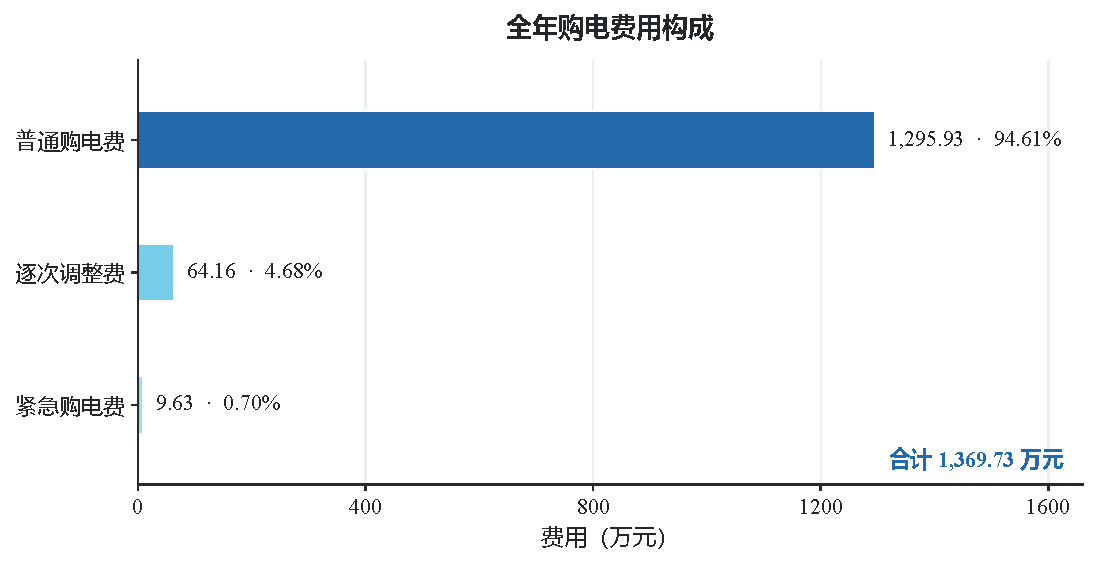
\includegraphics[width=0.88\textwidth]{../experiments/q3-models-20260911-04/figures/Fig2_Q3_CostBreakdown.pdf}}{}
\caption{问题三各路线的费用构成}\label{fig:q3-cost-local}
\end{figure}

% ==================================================

\section{问题四模型建立与求解}

\subsection{价格信息边界与任务分解}
附件4给出365天、每天144个10分钟区间的实际电价。题面没有说明未来价格发布时间，因此本文采用保守的因果信息边界：决策只能使用已经结束日期的电价；目标日真实价格仅在相应交易时段结算时进入账本。评价期仍为2025年2月1日至12月31日共334天。

问题4-2重新计算问题二，日内不修改计划；问题4-3重新计算问题三，在0:00、6:00、12:00和18:00更新当日剩余计划。两问共享光伏优先、储能边界、90\%充放电效率和5倍紧急购电规则，但使用各自的热启动状态和冻结参数。

\subsection{问题4-2：历史均价下的日前计划}
负载预测、光伏预测和净负荷余量沿用问题二的combined方案。每日0:00用此前7个完整日同一10分钟时段的均价形成$\widehat p_{d,t}^{(7)}$，并在当日144个区间上求解
\begin{equation}
 \min\sum_{t=1}^{144}\widehat p_{d,t}^{(7)}g_{d,t},
\end{equation}
约束仍为带符号净负荷下的供需平衡、光伏优先、储能递推及功率容量限制。富余光伏没有被截断为零，因此可直接进入充电约束。计划阶段要求日末储电量不低于1200 kWh；实际阶段使用真实负载、光伏和价格顺序执行，缺口才紧急购电。

模型曾比较固定价格曲线、7日均价、14日均价和供需残差SAA。修复光伏优先后，SAA全年费用14,523,376.59元，比7日均价低27,318.88元，但第三季度库存修正费用恶化0.37788\%，超过预先设置的0.1\%季度容许值。因此按预声明规则回退到7日均价方案。该门槛是团队选模规则，不是题目约束，也不能表述为7日均价具有最低全年费用。

\begin{table}[H]
\centering\small
\caption{问题4-2全年结果}\label{tab:q42-local}
\begin{tabular}{lr}
\toprule 指标 & 数值\\ \midrule
计划购电量/kWh & 21,599,339.14\\
计划购电费/元 & 14,013,336.77\\
紧急购电量/kWh & 89,217.88\\
紧急购电费/元 & 537,358.70\\
现金总费用/元 & \textbf{14,550,695.47}\\
库存价值修正后费用/元 & 14,557,043.61\\
期初/期末储电量/kWh & 10,800.00/1,488.80\\ \bottomrule
\end{tabular}
\end{table}

\begin{table}[H]
\centering\scriptsize
\caption{问题4-2指定日期结果}\label{tab:q42-dates-local}
\begin{tabular}{lrrrrr}
\toprule 日期 & 计划电量/kWh & 计划费/元 & 紧急电量/kWh & 总费用/元 & 日末SOC/kWh\\ \midrule
2025-03-20 & 69,027.33 & 43,376.68 & 35.58 & 43,612.01 & 1,550.51\\
2025-06-21 & 35,252.93 & 18,137.96 & 0 & 18,137.96 & 3,117.44\\
2025-09-23 & 70,396.09 & 46,525.85 & 0 & 46,525.85 & 3,015.19\\
2025-12-21 & 98,002.88 & 74,281.01 & 0 & 74,281.01 & 1,866.90\\ \bottomrule
\end{tabular}
\end{table}

\subsection{问题4-3：因果价格下的连续残差情景滚动}
问题4-3采用问题三相同的候选生成、场景回放和风险评分结构。1月1日以附件1价格曲线作为冷启动先验；此后使用此前最多14个完整日的同刻均价
\begin{equation}
 \widehat p_{d,t}=\max\left\{0.01,\frac1{|\mathcal D_d|}
 \sum_{j\in\mathcal D_d}p_{j,t}\right\},\qquad
 \mathcal D_d=\{\max(1,d-14),\ldots,d-1\}.
\end{equation}
每次发布时刻使用该预测价评价当日剩余区间的候选计划；当天未来及次日真实价格不进入计划。普通购电、调整费和紧急购电最终均按附件4交易时段真实价格结算。模型只优化至当天24:00，不能称为跨午夜未来24小时滚动优化。

\begin{table}[H]
\centering\small
\caption{问题4-3全年结果}\label{tab:q43-local}
\begin{tabular}{lr}
\toprule 指标 & 数值\\ \midrule
普通购电量/kWh & 20,946,711.61\\
普通购电费/元 & 13,646,853.14\\
调整费/元 & 675,169.92\\
紧急购电量/kWh & 19,840.03\\
紧急购电费/元 & 110,256.74\\
现金总费用/元 & \textbf{14,432,279.80}\\
库存价值修正后费用/元 & 14,432,805.82\\
日费用CVaR90/元 & 73,458.35\\
期初/期末储电量/kWh & 2,119.62/1,348.09\\ \bottomrule
\end{tabular}
\end{table}

CVaR90按334天等权经验分布最差10\%概率质量计算，即取最贵33天并加入第34贵日40\%的权重。该修正只改变风险汇总，不改变计划、逐日费用和全年现金总费用。

\begin{table}[H]
\centering\scriptsize
\caption{问题4-3指定日期结果}\label{tab:q43-dates-local}
\begin{tabular}{lrrrrrr}
\toprule 日期 & 普通电量/kWh & 普通费/元 & 调整费/元 & 紧急电量/kWh & 总费用/元 & 日末SOC/kWh\\ \midrule
2025-03-20 & 66,485.29 & 42,243.47 & 3,505.98 & 0 & 45,749.45 & 1,731.44\\
2025-06-21 & 34,618.52 & 17,597.33 & 627.81 & 0 & 18,225.13 & 2,549.48\\
2025-09-23 & 69,590.86 & 46,596.77 & 1,560.95 & 0 & 48,157.73 & 3,203.86\\
2025-12-21 & 95,497.74 & 71,954.50 & 3,561.88 & 43.05 & 75,819.12 & 1,493.63\\ \bottomrule
\end{tabular}
\end{table}

方向3相对同起点的旧余量滚动对照少支出171,182.49元，库存修正后少支出171,013.52元。问题4-2与4-3表面相差118,415.66元，但两者初始SOC、价格窗口、供需风险处理及调整权限不同，不能将该差额解释为日内预报收益。

\begin{figure}[H]
\centering
\IfFileExists{../deliverables/q4-3/figures/Fig2_Q4_3_CostBreakdown.pdf}{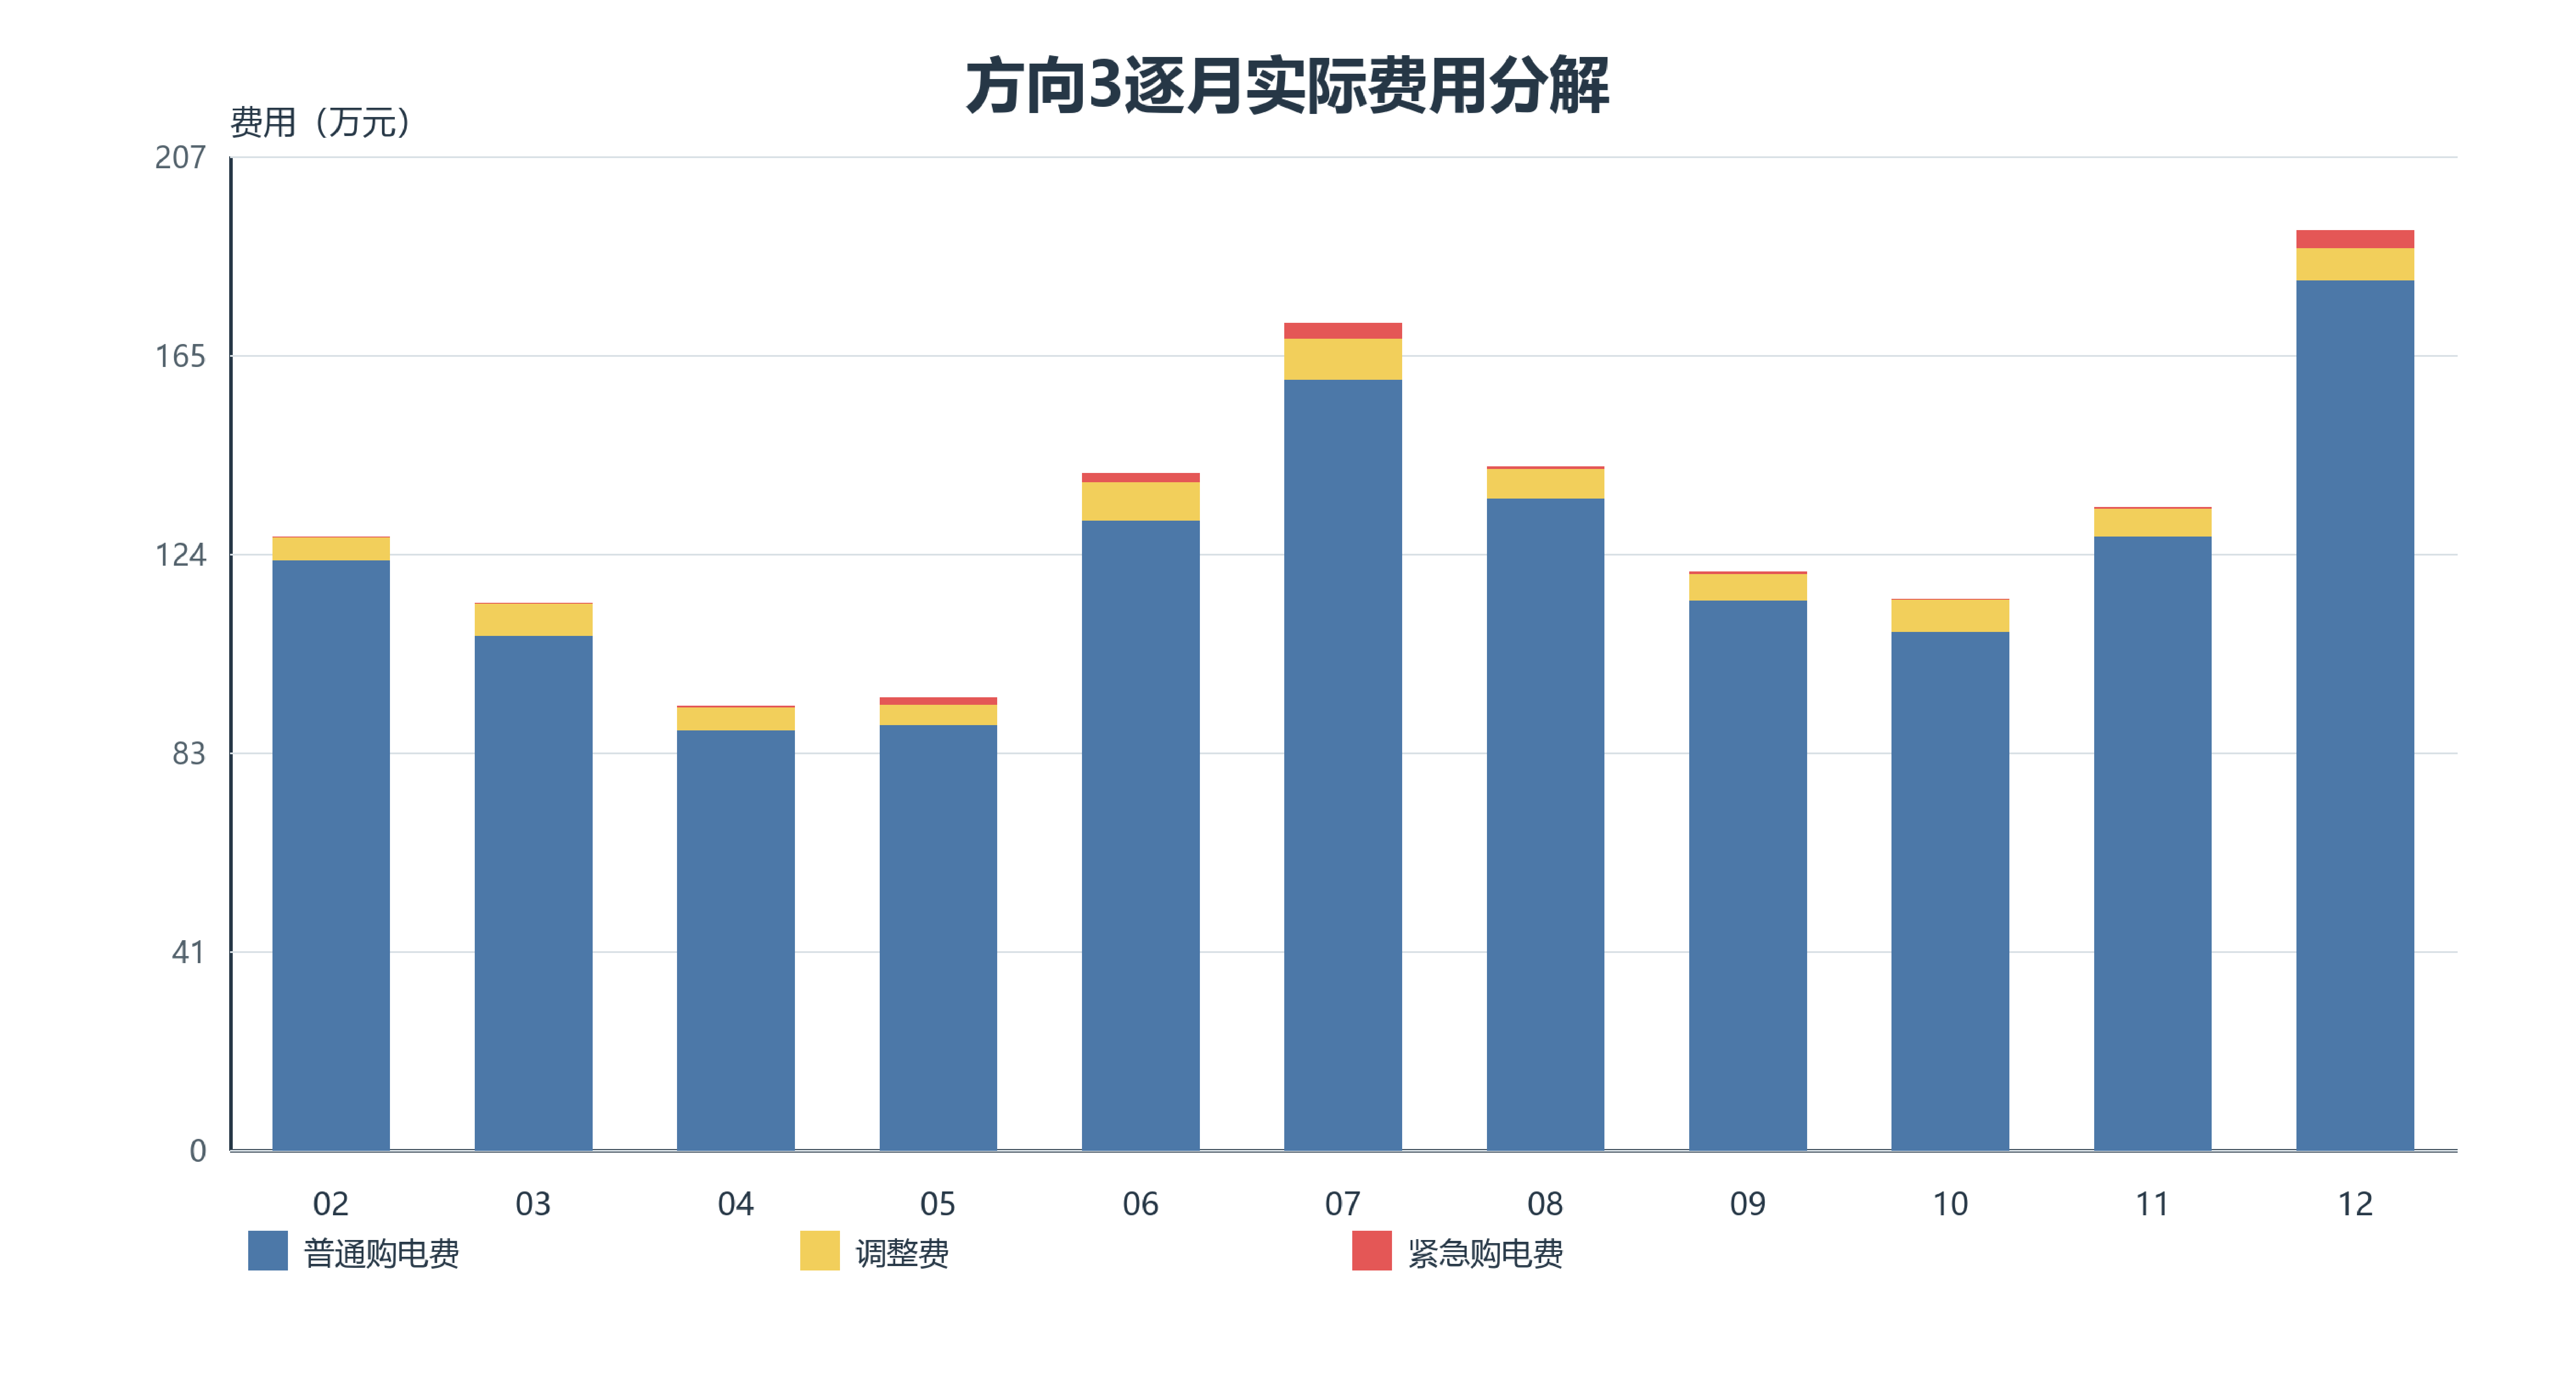
\includegraphics[width=0.88\textwidth]{../deliverables/q4-3/figures/Fig2_Q4_3_CostBreakdown.pdf}}{}
\caption{问题4-3方向3与余量对照的费用构成}\label{fig:q43-cost-local}
\end{figure}

\subsection{模型检验与适用范围}
问题4-2审计覆盖五种方法共240,480条执行记录、334个SAA计划、4,676条历史场景及1,336项未来价格扰动检查，独立复算通过，最大数值误差为$1.8233\times10^{-8}$。问题4-3共完成14,416次计划求解，其中LP 11,263次、MILP 3,153次；52,560条实际记录和1,460个计划版本通过原始输入、能量、SOC、费用、版本链、跨日连续及未来价格边界复算，最大状态误差为$9.095\times10^{-13}$ kWh。

问题4-3的旧84天预实验没有通过预声明门槛，而334天同起点回放优于旧余量对照；两者可以同时成立。全年结果支持当前交付选择，但不能据此证明收益必然来自残差时间相关性，也不能作为未知年份的外部验证。

% ==================================================

\section{模型检验与结果可靠性}

\subsection{问题一稳健性分析}

问题一将LP解重新代入144个区间的母线平衡和储能状态方程，并以完整MILP及独立重建LP
交叉核对；三种求解的费用均为35126.948589元，最大能量平衡残差为
$1.14\times10^{-13}$ kWh，库存递推误差为$1.82\times10^{-12}$ kWh，未出现同时充放电、
库存越界或光伏优先违规。

在电价、负载和设备参数不变的条件下，将光伏可用功率按$0\%$至$50\%$、步长$5\%$逐级削减并
重新求解。损失率为$0\%,5\%,10\%$时，最低购电费分别为35126.95、36697.19和38422.56元，
相对基准增加$0\%,4.47\%,9.38\%$；即使损失率达到$50\%$，模型仍得到可行解，储能相对无储能
情形的节约率仍为$17.22\%$。11组扰动均未出现同时充放电或约束违背，说明调度规则在光伏出力
偏差下保持可行，费用变化方向也符合供能规律。

\subsection{问题二稳健性分析}

问题二的独立审计覆盖18个候选、334天、144个日内区间，共865728条调度记录。
规划能量平衡、状态递推和光伏优先的最大误差分别不超过$4.77\times10^{-11}$、
$3.21\times10^{-10}$和$5.64\times10^{-9}$；实际执行能量平衡误差不超过
$4.55\times10^{-13}$。11项小实例及15项未来数据扰动检查均通过，表明费用计算、
跨日库存和历史信息边界与模型设定一致。

进一步分别扰动预测样本窗口、残差窗口、日末库存目标和规划时域。最终方案在2--4月、
5--8月和9--12月三个区间内的费用降幅分别为$15.04\%,12.31\%,13.86\%$，改善并未集中于
单一季节；将规划时域由24小时延长至48小时后，全年费用由13805129.20元变为13832749.53元，
相对变化仅$0.20\%$，且两种设置均满足能量平衡与库存边界。因此，问题二的主要结论对季节划分
和规划时域的小幅改变不敏感。

\subsection{问题三可靠性检验}
问题三主结果与输出工作簿由同一逐时段账本生成。方向3的334个评价日、48,096个执行区间及1,002次日内更新均完成；工作簿中的计划和调整计划各144时段与账本逐格一致，储能汇总和紧急购电明细完整。六策略联合独立审计覆盖315,360条执行记录与7,650次版本更新，能量守恒、SOC边界、跨日连续、逐次调整费和未来数据扰动检查均通过。

\subsection{问题四可靠性检验}
问题4-2以预先冻结的季度稳定性规则进行模型选择。SAA全年现金费用低于mean7，但第三季度库存修正费用超过较优基线0.37788\%，因此回退mean7；这一结论是选择规则的结果，并不表示SAA求解或物理约束失败。

问题4-3除现金总费用外，报告73,458.35元的日费用CVaR90。该指标直接由334天逐日现金费用按等权经验分布计算，用于描述高费用日期的尾部水平；本文没有实施“风险压降25\%”约束，也不使用紧急购电总量代替尾部风险指标。价格后缀和未来负载扰动不改变相应决策时刻的预测输入，信息因果检查通过。

% ==================================================

\section{模型评价、改进与推广}

\subsection{模型优点}
四问共享相同的能量守恒、储能状态和因果执行内核。问题三通过连续历史残差保留误差的时序形态，同时让每个候选计划在所有情景中固定，再以同一执行器评价，降低场景内预见性偏差。问题四明确区分决策价格和结算价格，所有未来信息扰动均可复算；费用、库存和版本链均由逐时段账本汇总。

\subsection{模型局限}
问题三和4-3只优化到当日24:00，未利用附件3跨日至未来24小时的完整窗口。连续残差情景只有8条，CVaR评分反映有限历史样本，并非真实分布的精确估计。问题4-2与4-3采用不同价格窗口和热启动接口，不能用两者总费用差直接归因于日内预报。现有实验是2025年按时间顺序的历史回放，不是未知年份盲测。

\subsection{改进方向}
可在保持逐次结算口径的前提下把预测窗口扩展至未来24小时，只对当天已申报后缀收取调整费；还可固定起点、供需预测、价格预测和执行器，分别进行残差路径时序打乱、情景数和风险权重对照，以识别时间相关性及日内预报的独立贡献。

% ==================================================
\section{结论}
\begin{enumerate}[label=\textbf{问题\chinese*：},leftmargin=5.5em]
  \item 在附件1预测、区间末值映射及$E_0=E_{144}=6000$ kWh条件下，最优全天购电量为59482.698998 kWh，购电费用为35126.948589元。
  \item 以1月为热启动期、2月至12月为评价期，问题二combined方案现金总费用为1380.5129万元，其中计划电费1329.9833万元、紧急电费50.5296万元。
  \item 问题三方向3的普通购电费、调整费和紧急购电费分别为1295.9331万元、64.1629万元和9.6296万元，现金总费用为1369.7255万元；相对方向2减少15.4917万元。该优势来自整体策略差异，未单独归因于新增预报。
  \item 问题4-2采用过去7日同刻均价预测，现金总费用为1455.0695万元；问题4-3采用过去14日同刻均价与连续残差情景滚动，现金总费用为1443.2280万元，日费用CVaR90为7.3458万元。两套结果均不使用当天未来或次日真实价格进行决策。
\end{enumerate}

% ==================================================

\section*{参考文献}
\addcontentsline{toc}{section}{参考文献}
\begin{enumerate}[label={\textnormal{[\arabic*]}},leftmargin=3em]
  \item Dantzig G B, Orden A, Wolfe P. The generalized simplex method for minimizing a linear form under linear inequality restraints[J]. Pacific Journal of Mathematics, 1955, 5(2): 183--195.
  \item Rockafellar R T, Uryasev S. Optimization of conditional value-at-risk[J]. Journal of Risk, 2000, 2(3): 21--41.
\end{enumerate}

% ==================================================

\section*{附录}
\addcontentsline{toc}{section}{附录}

\subsection*{附录一：附件表}



\subsection*{附录二：代码表}
问题一线性规划核心代码
\begin{lstlisting}[language=Python]
from pathlib import Path
import sys
import numpy as np
import openpyxl
from scipy.optimize import linprog


def solve_q1_lp(input_xlsx):
    """Q1 LP. All bus-side flows are in kWh."""
    book = openpyxl.load_workbook(
        Path(input_xlsx), read_only=True, data_only=True
    )
    data = np.array(
        [row[1:] for row in book.active.iter_rows(
            min_row=2, values_only=True
        )],
        dtype=float,
    )
    book.close()

    price, load_kw, pv_kw = data.T
    load = load_kw / 6.0
    pv = pv_kw / 6.0
    n = len(price)
    eta = 0.9
    slot_limit = 5000.0 / 6.0

    # x = [grid, charge, discharge, curtailment, E_0, ..., E_T]
    size = 5 * n + 1
    objective = np.zeros(size)
    objective[:n] = price
    a_eq, b_eq = [], []

    for t in range(n):
        # grid + pv + discharge = load + charge + curtailment
        row = np.zeros(size)
        row[t] = 1.0
        row[n + t] = -1.0
        row[2 * n + t] = 1.0
        row[3 * n + t] = -1.0
        a_eq.append(row)
        b_eq.append(load[t] - pv[t])

        # E_(t+1) = E_t + eta*charge - discharge/eta
        row = np.zeros(size)
        row[4 * n + t + 1] = 1.0
        row[4 * n + t] = -1.0
        row[n + t] = -eta
        row[2 * n + t] = 1.0 / eta
        a_eq.append(row)
        b_eq.append(0.0)

    surplus = np.maximum(pv - load, 0.0)
    deficit = np.maximum(load - pv, 0.0)
    bounds = []
    bounds += [(0.0, None)] * n
    bounds += [(0.0, slot_limit)] * n
    bounds += [(0.0, min(slot_limit, value)) for value in deficit]
    bounds += [(0.0, value) for value in surplus]
    bounds += [(1200.0, 10800.0)] * (n + 1)
    bounds[4 * n] = (6000.0, 6000.0)
    bounds[-1] = (6000.0, 6000.0)

    result = linprog(
        objective,
        A_eq=np.asarray(a_eq),
        b_eq=np.asarray(b_eq),
        bounds=bounds,
        method="highs",
    )
    if not result.success:
        raise RuntimeError(result.message)

    grid = result.x[:n]
    charge = result.x[n:2*n]
    discharge = result.x[2*n:3*n]
    curtailment = result.x[3*n:4*n]
    energy = result.x[4*n:]

    tol = 1e-6
    balance = grid + pv + discharge - load - charge - curtailment
    state_error = np.diff(energy) - eta * charge + discharge / eta
    assert np.max(np.abs(balance)) <= tol
    assert np.max(np.abs(state_error)) <= tol
    assert not np.any((charge > tol) & (discharge > tol))

    return result.fun, grid, charge, discharge, curtailment, energy


if __name__ == "__main__":
    cost, grid, charge, discharge, curtailment, energy = \
        solve_q1_lp(sys.argv[1])
    print(f"cost_yuan={cost:.6f}")
    print(f"purchase_kwh={grid.sum():.6f}")
    print(f"curtailment_kwh={curtailment.sum():.6f}")
    print(f"E0={energy[0]:.6f}, E24={energy[-1]:.6f}")
\end{lstlisting}

问题二预测与因果执行核心代码

\begin{lstlisting}[language=Python]
from datetime import date
import numpy as np


def predict(load, pv, dates, i):
    """Past-only weekday load forecast and seven-day PV mean."""
    weekday = date.fromisoformat(dates[i]).weekday()
    indices = [
        j for j in range(max(0, i - 35), i)
        if date.fromisoformat(dates[j]).weekday() == weekday
    ]
    if len(indices) < 2:
        indices = list(range(max(0, i - 7), i))
    load_hat = load[indices].mean(axis=0)
    pv_hat = pv[max(0, i - 7):i].mean(axis=0)
    return load_hat, pv_hat


def safety_margin(past_residuals, q=0.8, days=14,
                  bucket_slots=6, slots=144):
    """Hourly pooled positive quantile of past net-load errors."""
    if not len(past_residuals):
        return np.zeros(slots)
    errors = np.asarray(past_residuals[-days:])
    values = [
        max(0.0, float(np.quantile(
            errors[:, t:t + bucket_slots], q, method="linear"
        )))
        for t in range(0, slots, bucket_slots)
    ]
    return np.repeat(values, bucket_slots)


def causal_step(plan_kwh, load_kwh, pv_kwh, energy, cfg):
    """Execute one slot using no future actual observation."""
    eta = cfg["charge_efficiency"]
    eta_d = cfg["discharge_efficiency"]
    cap = cfg["power_kw"] * cfg["step_hours"]
    e_min, e_max = cfg["energy_min"], cfg["energy_max"]

    pv_load = min(load_kwh, pv_kwh)
    grid_load = min(plan_kwh, load_kwh - pv_load)
    shortage = max(0.0, load_kwh - pv_load - grid_load)
    if shortage > 0:
        discharge = min(shortage, cap, max(0.0, energy-e_min)*eta_d)
        emergency = shortage - discharge
        pv_charge = grid_charge = 0.0
    else:
        room = min(cap, max(0.0, e_max-energy)/eta)
        pv_charge = min(pv_kwh-pv_load, room)
        grid_charge = min(plan_kwh-grid_load, room-pv_charge)
        discharge = emergency = 0.0

    charge = pv_charge + grid_charge
    energy_next = energy + eta*charge - discharge/eta_d
    unused_plan = max(0.0, plan_kwh-grid_load-grid_charge)
    return energy_next, emergency, charge, discharge, unused_plan


def run_day(price, plan_kwh, actual_load, actual_pv, energy, cfg):
    rows = []
    for t in range(144):
        result = causal_step(
            plan_kwh[t], actual_load[t], actual_pv[t], energy, cfg
        )
        energy, emergency, charge, discharge, unused = result
        rows.append({
            "slot": t,
            "plan_kwh": plan_kwh[t],
            "emergency_kwh": emergency,
            "charge_kwh": charge,
            "discharge_kwh": discharge,
            "paid_grid_spill_kwh": unused,
            "cost": price[t]*plan_kwh[t]
                    + 5.0*price[t]*emergency,
            "e_end": energy,
        })
    return rows, energy
\end{lstlisting}

问题三和问题四的论文结果直接由仓库程序生成。为避免再次出现附录摘录与真实程序不同步，以下代码从仓库源文件按行引用。

\subsubsection*{问题三预测读取与光伏插值}
\lstinputlisting[language=Python,firstline=21,lastline=116]{../scripts/q3_shared.py}

\subsubsection*{问题三计划优化、逐次调整费与CVaR评分}
\lstinputlisting[language=Python,firstline=24,lastline=177]{../scripts/q3_core.py}

\subsubsection*{问题三滚动运行与结果汇总}
\lstinputlisting[language=Python,firstline=130,lastline=268]{../scripts/run_q3_models.py}

\subsubsection*{问题4-2历史价格预测与日前执行}
\lstinputlisting[language=Python,firstline=43,lastline=158]{../scripts/run_q4_saa_full.py}

\subsubsection*{问题4-3因果电价与连续残差情景滚动}
\lstinputlisting[language=Python,firstline=95,lastline=330]{../scripts/run_q4_3_scenario_full.py}

\end{document}
